% Chapter 1
%\chapter{مقدمه}

\section{مقدمه}
یادگیری فدرال

\section{کارهای مرتبط}

\subsection{
	روش جابه‌جایی فدرال%
	\LTRfootnote{Federated Swapping}
	\lr{\texttt{\fontspec{Times New Roman} (FedSwap)}}
}
در این روش، یک عملیات جدید به نام جابه‌جایی فدرال یا
\lr{FedSwap}
پیشنهاد شده است که به عنوان جایگزینی برای برخی از دوره‌های
\lr{FedAvg}
در یادگیری فدرال به کار می‌رود.
این عملیات با هدف بهبود فرآیند یادگیری فدرال و کاهش تاثیرات منفی داده‌های
\lr{non-IID}
طراحی شده است
\cite{chiu2020semisupervised}.


در روش‌ یادگیری فدرال، پس از هر تکرار، مدل‌های محلی از دستگاه‌های نهایی جمع‌آوری شده و یک مدل جامع از ترکیب آن‌ها ساخته می‌شود. اما در روش
\lr{FedSwap}%
، به‌جای این که این ادغام در هر تکرار انجام شود، سرور مدل‌های محلی را در گام‌های مشخصی بین دستگاه‌ها جابه‌جا می‌کند. در واقع، در انتهای برخی مراحل، عملیات جابه‌جایی و در انتهای برخی دیگر، ادغام مدل‌ها صورت می‌گیرد. این مراحل بر اساس پارامترهایی که به عنوان ورودی تعریف می‌شوند، تعیین می‌گردند.
جهت درک بهتر این ساختار به شکل
\ref{federated_swapping}
توجه نمایید.


\begin{figure}[t]
	\centering
	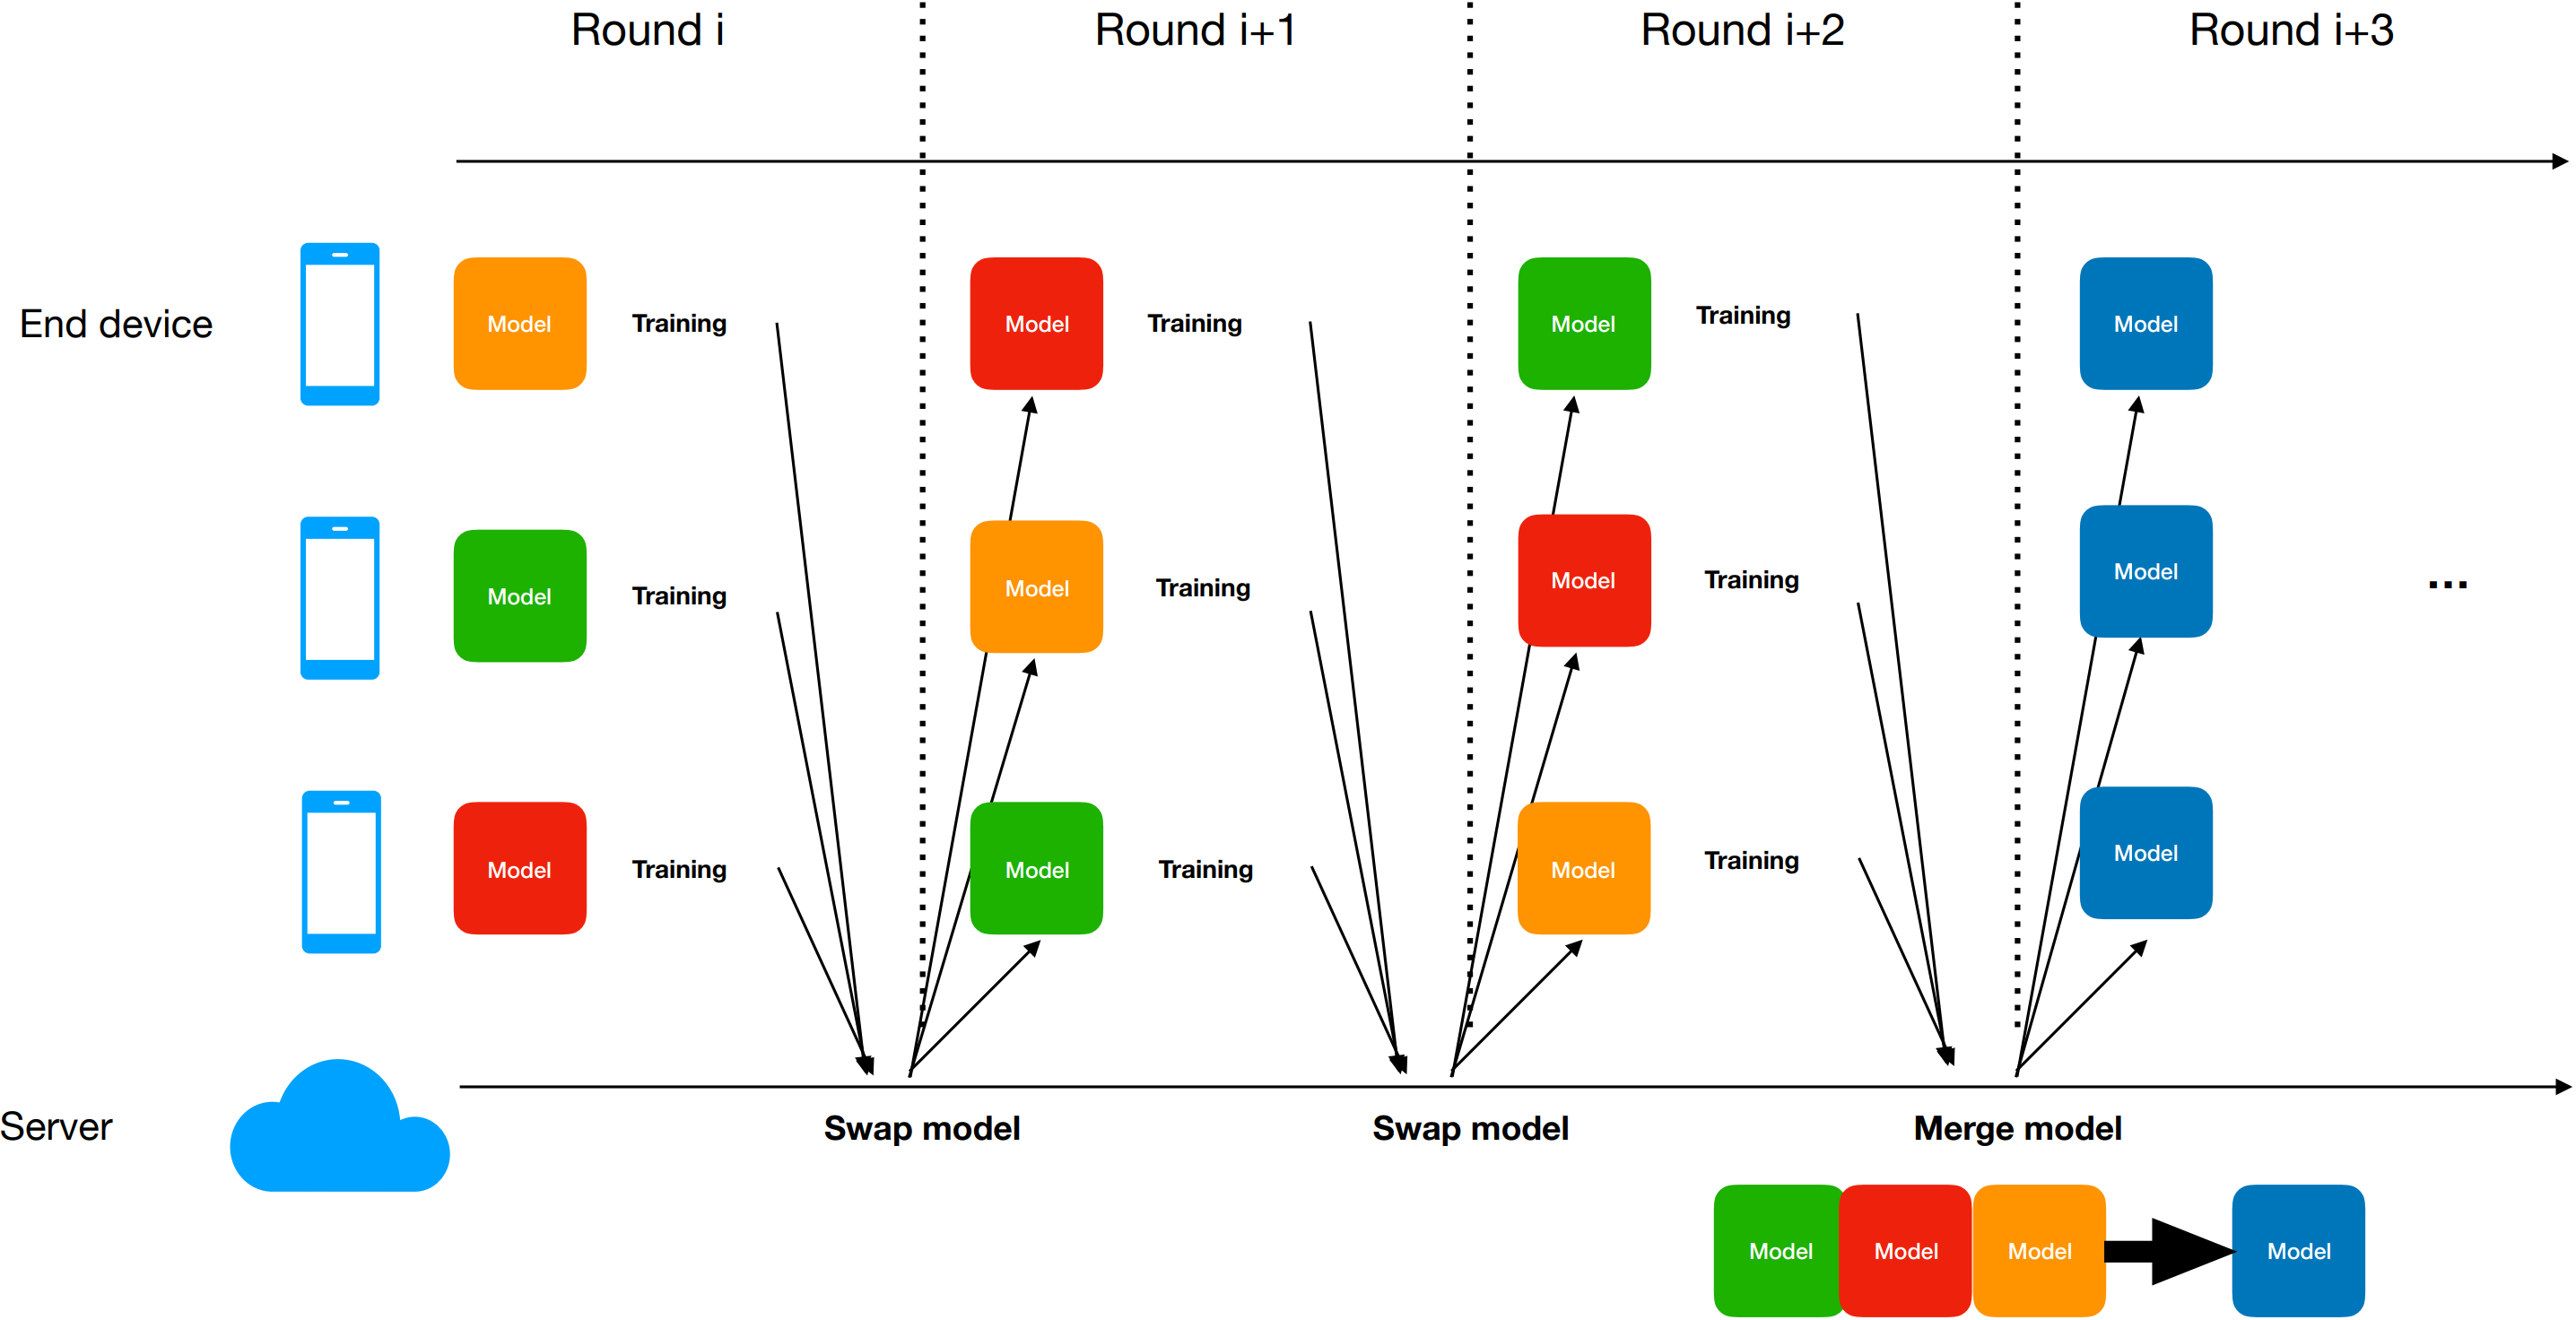
\includegraphics[scale=0.179]{images/chap4/federated_swapping.png}%
	\caption{%
		روش جابه‌جایی فدرال
		\cite{chiu2020semisupervised}%
		.
	}
	\label{federated_swapping}
	\centering
\end{figure}








\subsection{معیارهای مشابهت}

 فرض کنید \( X \) ماتریسی با ابعاد \( n \times p_1 \) باشد که \( X \in \mathbb{R}^{n \times p_1} \) شامل \( n \) نمونه و \( p_1 \) ویژگی است. همچنین، \( Y \) ماتریسی با ابعاد \( n \times p_2 \) باشد که \( Y \in \mathbb{R}^{n \times p_2} \) شامل \( n \) نمونه و \( p_2 \) ویژگی است. فرض می‌شود که \( p_1 \) کمتر یا مساوی \( p_2 \) است.
 
 
 هدف طراحی و تحلیل یک شاخص شباهت عددی \( s(X, Y) \) است که بتواند بازنمایی‌های%
 \LTRfootnote{Representations}
 موجود در ماتریس‌های \( X \) و \( Y \) را هم درون یک شبکه عصبی و هم بین شبکه‌های عصبی مختلف مقایسه کند. چنین شاخصی به درک بهتر تأثیر عوامل مختلف در یادگیری عمیق کمک می‌کند.
 
 به عنوان مثال، در بررسی شبکه‌های عصبی، ماتریس \( X \) می‌تواند نمایانگر فعال‌سازهای%
 \LTRfootnote{Activations}
 نورون‌ها در یک لایه خاص برای \( n \) نمونه ورودی باشد و ماتریس \( Y \) می‌تواند نمایانگر فعال‌سازهای نورون‌ها در لایه‌ای دیگر یا حتی در یک شبکه عصبی دیگر برای همان \( n \) نمونه باشد. مقایسه این دو ماتریس اطلاعات مهمی درباره نحوه یادگیری و بازنمایی داده‌ها توسط شبکه عصبی ارائه می‌دهد.
 
 
******
 در این بخش به بررسی روش‌های مختلفی که برای سنجش مشابهت بین بازنمایی‌های شبکه‌های عصبی استفاده می‌شود، پرداخته خواهد شد. یکی از روش‌های مهم در این زمینه استفاده از پایه‌های متعامد است. به‌طور خاص، فرض می‌شود که \( Q_X \) و \( Q_Y \) پایه‌های متعامدی برای ستون‌های ماتریس‌های \( X \) و \( Y \) هستند. به این معنا که \( Q_X \) و \( Q_Y \) به‌صورت \( Q_X = X(X^T X)^{-1/2} \) و \( Q_Y = Y(Y^T Y)^{-1/2} \) تعریف شده‌اند. این پایه‌های متعامد امکان تحلیل مؤثرتر بازنمایی‌های شبکه عصبی و سنجش دقیق‌تر شباهت‌های آن‌ها را فراهم می‌کنند.
 تمامی رابطه‌های مورد استفاده در بخش
 \ref{sec_similarity_measurement_criteria}%
 ، از مرجع 
 \cite{kornblith2019similarity} 
 برگرفته شده‌اند.
 
 
 
 
 \subsection{
 	قرینه مجموع اختلاف مطلق%
 	\LTRfootnote{Opposite Sum of Absolute Difference}
 	\lr{\texttt{\fontspec{Times New Roman} (OSAD)}}
 }
 معیار سنجش شباهت باید به گونه‌ای تعریف شود که علاوه بر داشتن پایداری در مقابل تبدیل‌های متعامد و مقیاس‌بندی یکسان، قادر باشد ماتریس‌هایی با ابعاد مختلف را نیز پوشش دهد. با این حال، در صورتی که فرض شود ماتریس‌های مورد بررسی دارای ساختار یکسان و ابعاد ثابت هستند و همچنین مقدار‌های اولیه این ماتریس‌ها یکسان در نظر گرفته شوند، می‌توان از معیار
 \lr{OSAD}
 استفاده نمود.
 
 در صورتی که ابعاد به شکل \( n \times p \) تعریف شوند، از رابطه زیر برای مقایسه و اندازه‌گیری شباهت استفاده می‌شود:
 \begin{equation}
 	OSAD = -\sum_{i=1}^n \sum_{j=1}^{p_1} Z_{ij}
 	\quad \text { where } \quad
 	Z = |X-Y|
 \end{equation}
 
 در این رابطه، \( X \) و \( Y \) ماتریس‌های ورودی هستند و \( Z \) ماتریسی است که از اختلاف مطلق بین این دو به دست می‌آید. در نهایت قرینه مجموع مقادیر ماتریس \( Z \) که با
 \lr{OSAD}
 نشان داده می‌شود، به عنوان معیاری برای سنجش میزان شباهت مورد استفاده قرار می‌گیرد.
 
 با توجه به این که در این روش فرض بر این است که ابعاد ماتریس‌ها و مقدار‌های اولیه ثابت و یکسان هستند، معیار
 \lr{OSAD}
 به عنوان ابزاری مفید و قابل اعتماد برای مقایسه و ارزیابی شباهت بین دو ماتریس مختلف مطرح می‌شود. این معیار به سادگی اختلاف‌های موجود در مقادیر را محاسبه کرده و قرینه مجموع آن‌ها را به عنوان نتیجه ارائه می‌دهد، که در تحلیل‌های مختلف بسیار کاربردی خواهد بود.
 
 
 
 
 \subsection{
 	تحلیل همبستگی کانونی%
 	\LTRfootnote{Canonical Correlation Analysis}
 	\lr{\texttt{\fontspec{Times New Roman} (CCA)}}
 }
 برای درک بهتر تحلیل همبستگی کانونی، از یک مثال ساده استفاده می‌شود. فرض کنید دو مجموعه داده مختلف در اختیار است، مجموعه‌ای شامل اطلاعاتی همچون قد و وزن افراد و مجموعه دیگر حاوی اطلاعاتی مانند سن و درآمد آن‌ها باشد. هدف تحلیل همبستگی کانونی، این است که ارتباط‌های پنهان بین این دو مجموعه داده را کشف کند. به بیان ساده،
 \lr{CCA}
 به دنبال شناسایی ترکیب‌هایی از ویژگی‌ها در هر مجموعه داده است که با مقایسه آن‌ها، بیشترین همبستگی حاصل شود. تلاش بر این است که مشخص شود کدام ترکیب قد و وزن با کدام ترکیب سن و درآمد بیشترین ارتباط را دارد.
 
 ابتدا داده‌ها استاندارد می‌شوند، به این صورت که میانگین هر ویژگی صفر شده و داده‌ها به گونه‌ای تغییر می‌کنند که انحراف معیارشان یک شود. سپس،
 \lr{CCA}
 بردارهای وزنی را برای هر مجموعه داده محاسبه می‌کند تا ترکیب‌های خطی از این داده‌ها ایجاد کند. این ترکیب‌ها به گونه‌ای انتخاب می‌شوند که حداکثر همبستگی بین آن‌ها وجود داشته باشد. به عنوان مثال،
 \lr{CCA}
 می‌خواهد ترکیبی از قد و وزن (مثلاً \(0.5 \times \text{قد} + 0.5 \times \text{وزن}\)) و ترکیبی از سن و درآمد (مثلاً \(0.3 \times \text{سن} + 0.7 \times \text{درآمد}\)) را بیابد که بیشترین ارتباط را با هم داشته باشند.
 
 با استفاده از این بردارهای وزنی، ترکیب‌های جدیدی از داده‌ها ایجاد می‌شوند و سپس همبستگی بین این ترکیب‌ها محاسبه می‌شود.
 \lr{CCA}
 به دنبال یافتن پایه‌هایی برای دو ماتریس است به طوری که وقتی ماتریس‌های اصلی بر روی این پایه‌ها توزیع می‌شوند، همبستگی به حداکثر برسد. برای هر \(i\) که بین 1 تا \(p_1\) (تعداد ویژگی‌ها) قرار دارد، ضریب همبستگی کانونی \( \rho_i \) به‌صورت زیر تعریف می‌شود: 
 \begin{equation}
 	\rho_i = \max_{\mathbf{w}_X^i, \mathbf{w}_Y^i} \text{corr}(X \mathbf{w}_X^i, Y \mathbf{w}_Y^i)
 \end{equation}
 با در نظر گرفتن بردارهای \(\mathbf{w}_X^i \in \mathbb{R}^{p1}\) و \(\mathbf{w}_Y^i \in \mathbb{R}^{p2}\)، ضریب همبستگی کانونی \( \rho_i \) هدفش این است که همبستگی بین ترکیب خطی \( X \mathbf{w}_X^i \) و \( Y \mathbf{w}_Y^i \) را به حداکثر برساند.
 
 برای اطمینان از این که ترکیب‌های جدید داده‌ها مستقل و متفاوت از هم باشند، شرط‌های زیر باید رعایت شوند:
 \begin{equation}
 	\begin{array}{ll}
 		\forall_{j<i} & X \mathbf{w}_X^i \perp X \mathbf{w}_X^j
 		\\
 		\\
 		\forall_{j<i} & Y \mathbf{w}_Y^i \perp Y \mathbf{w}_Y^j
 	\end{array}
 \end{equation}
 این شرط‌ها اطمینان می‌دهند که ترکیب‌های جدید از داده‌ها با ترکیب‌های قبلی همپوشانی نداشته و متعامد باقی بمانند.
 
 در نهایت برای مقایسه دو شبکه عصبی و اندازه‌گیری شباهت بین آن‌ها، از معیاری به نام \( R^2_{CCA} \) استفاده می‌شود. این معیار نشان می‌دهد که چقدر از اطلاعات داده‌ها، توسط ترکیب‌های خطی حاصل از روش
 \lr{CCA}
 توضیح داده می‌شود. رابطه این معیار به این صورت است:
 \begin{equation}
 	R^2_{CCA} = \frac{\sum_{i=1}^{p1} \rho^2_i}{p1} = \frac{||Q^T_Y Q_X||^2_F}{p1}
 	\label{eq_CCA}
 \end{equation}
 که با محاسبه و جمع کردن مربعات ضرایب همبستگی کانونی و سپس تقسیم آن‌ها بر تعداد ضرایب، میزان شباهت بین دو شبکه عصبی را ارزیابی می‌کند.
 
 با استفاده از روش
 \lr{CCA}%
 ، می‌توان ترکیب‌های خطی از ویژگی‌های دو مجموعه داده مختلف را شناسایی کرد که بالاترین همبستگی را با هم دارند. این روش کمک می‌کند تا روابط پنهان و مهم بین هر دو مجموعه داده آشکار شود و تحلیل‌های دقیق‌تری صورت گیرد.
 
 
 
 
 
 
 
 \subsection{
 	معیار استقلال هیلبرت-اشمیت%
 	\LTRfootnote{Hilbert-Schmidt Independence Criterion}
 	\lr{\texttt{\fontspec{Times New Roman} (HSIC)}}
 }
 برای بررسی میزان وابستگی و شباهت بین دو مجموعه داده، می‌توان از معیار استقلال هیلبرت-اشمیت استفاده کرد. این معیار به‌طور خاص برای اندازه‌گیری همبستگی بین داده‌های مختلف طراحی شده است. به‌طور دقیق‌تر، برای داده‌های مرکزیت‌یافته (میانگین صفر در هر ستون) \(X\) و \(Y\)، رابطه زیر برقرار است:
 \begin{equation}
 	\frac{1}{(n - 1)^2} \text{tr}(XX^TYY^T) = ||\text{cov}(X^T, Y^T)||_F^2
 \end{equation}
 
 معیار
 \lr{HSIC}
 این معادله را با استفاده از فضایی خاص تعمیم می‌دهد و امکان بررسی مؤثر وابستگی‌ها را فراهم می‌کند. به بیان دیگر، این معیار با بهره‌گیری از توابع هسته‌ای، همبستگی بین ماتریس‌های داده را اندازه‌گیری می‌کند. به این نحو که عناصر \(K_{ij}\) و \(L_{ij}\) به ترتیب از طریق \(k(x_i, x_j)\) و \(l(y_i, y_j)\) محاسبه می‌شوند، که در این‌جا \(k\) و \(l\) توابع هسته‌ای هستند
 \cite{gretton2005measuring}.
 
 برآورد
 \lr{HSIC}
 به‌صورت زیر تعریف می‌شود:
 \begin{equation}
 	\text{HSIC}(K, L) = \frac{1}{(n - 1)^2} \text{tr}(KHLH)
 	\label{eq_HSIC}
 \end{equation}
 که در آن
 \(H\)
 ماتریس مرکزیت‌دهنده است و به شکل \(H_n = I_n - \frac{1}{n} 11^T\) تعریف می‌شود.
 
 نکته جالب این است که اگر هسته‌های خطی \(k\) و \(l\) به‌صورت \(k(x, y) = l(x, y) = x^Ty\) باشند،
 \lr{HSIC}
 به همان معادله اولیه برمی‌گردد. این بدین معناست که معیار 
 \lr{HSIC} 
 به‌طور دقیق و قابل اعتماد، میزان وابستگی و شباهت بین داده‌ها را ارزیابی کرده و به درک بهتر ساختارهای پیچیده داده‌ها کمک می‌کند.
 
 
 \subsection{
 	هم‌ترازی هسته مرکزی%
 	\LTRfootnote{Centered Kernel Alignment}
 	\lr{\texttt{\fontspec{Times New Roman} (CKA)}}
 }
 معیار
 \lr{HSIC}
 در اندازه‌گیری همبستگی‌ها با مشکل عدم پایداری نسبت به مقیاس‌بندی یکسان ویژگی‌ها مواجه است. این بدان معناست که در صورت تغییر مقیاس ویژگی‌ها، نتیجه
 \lr{HSIC}
 ممکن است دچار تغییراتی شود که به درستی شباهت‌های بین داده‌ها را نشان ندهد. برای رفع این مورد، از فرم نرمال‌شده‌ای به نام هم‌ترازی هسته مرکزی استفاده می‌شود.
 
 در حقیقت
 \lr{CKA}
 یک شاخص نرمال‌ شده است که تأثیر مقیاس‌بندی یکسان را حذف می‌کند و به این ترتیب، دقت و پایداری بیشتری در مقایسه بازنمایی‌های شبکه‌های عصبی فراهم می‌آورد
 \cite{cortes2012algorithms, cristianini2001kernel}.
 رابطه
 \lr{CKA}
 به شکل زیر تعریف می‌شود:
 \begin{equation}
 	\text{CKA}(K, L) = \frac{\text{HSIC}(K, L)}{\sqrt{\text{HSIC}(K, K) \cdot \text{HSIC}(L, L)}}
 	\label{eq_CKA}
 \end{equation}
 که در آن عبارت \(\text{HSIC}(K, L)\) میزان همبستگی بین دو ماتریس هسته‌ای \(K\) و \(L\) را اندازه‌گیری می‌کند. صورت کسر، همان
 \lr{HSIC}
 اصلی است که میزان همبستگی بین دو ماتریس داده را نشان می‌دهد. اما برای نرمال‌سازی این مقدار و حذف تأثیر مقیاس‌بندی، مخرج کسر به کار می‌رود که شامل ضرب دو
 \lr{HSIC}
 مربوط به هر یک از ماتریس‌ها با خودشان است. این نرمال‌سازی باعث می‌شود که نتیجه نهایی مستقل از مقیاس‌بندی ویژگی‌ها باشد و شباهت‌های واقعی بین داده‌ها را بهتر منعکس کند.
 
 استفاده از
 \lr{CKA}
 در مقایسه با
 \lr{HSIC}%
 ، به‌ویژه در تحلیل بازنمایی‌های شبکه‌های عصبی و داده‌های پیچیده، کارایی بهتری دارد. زیرا این شاخص نرمال‌شده، نه تنها شباهت‌های بین داده‌ها را دقیق‌تر می‌سنجد، بلکه در برابر تغییرات مقیاس‌بندی نیز مقاوم است. به این ترتیب، می‌توان از
 \lr{CKA}
 به عنوان یک ابزار قدرتمند برای درک و تحلیل بازنمایی‌های مختلف در یادگیری عمیق و دیگر زمینه‌های مرتبط استفاده کرد.
 
 
 
 
 \subsection{
 	هم‌ترازی هسته مرکزی بدون مداخله%
 	\LTRfootnote{Deconfounded Centered Kernel Alignment}
 	\lr{\texttt{\fontspec{Times New Roman} (dCKA)}}
 }\label{sec_dCKA}
 فرض می‌شود \(X\) یک مجموعه داده ورودی با \(n\) نمونه و \(p\) ویژگی باشد. نمایش‌ لایه‌های \(m_1\) و \(m_2\) از دو شبکه عصبی که به ترتیب \(f_1\) و \(f_2\) نامیده می‌شوند، به‌صورت \(X^{m_1}_{f_1}\) و \(X^{m_2}_{f_2}\) هستند. شبکه‌های عصبی \(f_1\) و \(f_2\) دو مدل متفاوت یادگیری ماشین با معماری و ساختار مخصوص به خود هستند. لایه‌های \(m_1\) و \(m_2\) نیز لایه‌های خاصی در این شبکه‌ها هستند که مورد بررسی قرار می‌گیرند. برای مثال، \(m_1\) می‌تواند لایه دوم از شبکه \(f_1\) و \(m_2\) می‌تواند لایه چهارم از شبکه \(f_2\) باشد
 \cite{cui2022deconfounded}.
 تمامی رابطه‌های مورد استفاده در بخش
 \ref{sec_dCKA}%
 ، از مرجع 
 \cite{cui2022deconfounded} 
 برگرفته شده‌اند.
 
 برای مقایسه نمایش‌های دو شبکه عصبی، ساختارهای شباهت در هر شبکه بررسی می‌شود. این کار با محاسبه شباهت بین هر جفت از نمونه‌ها در \(X^{m_1}_{f_1}\) و \(X^{m_2}_{f_2}\) با استفاده از یک معیار شباهت \( k(\cdot, \cdot) \) انجام می‌شود:
 \begin{equation}
 	K^{m_1}_{f_1} = k(X^{m_1}_{f_1}, X^{m_1}_{f_1}), \quad K^{m_2}_{f_2} = k(X^{m_2}_{f_2}, X^{m_2}_{f_2})
 	\label{eq_dCKA_Kernel}
 \end{equation}
 در این رابطه ماتریس‌های \(K^{m_1}_{f_1}\) و \(K^{m_2}_{f_2}\) نشان‌دهنده شباهت بین هر جفت از نمونه‌ها در لایه‌های \(m_1\) و \(m_2\) از شبکه‌های \(f_1\) و \(f_2\) هستند. در مرحله بعد، برای مقایسه این دو ماتریس از معیاری به نام \(s(\cdot, \cdot)\) استفاده می‌شود:
 \begin{equation}
 	s^{m_1,m_2}_{f_1,f_2} = s(K^{m_1}_{f_1}, K^{m_2}_{f_2})
 	\label{eq_similarity}
 \end{equation}
 این مقدار بیانگر میزان شباهت بین دو نمایش شبکه‌های عصبی است
 \cite{cui2022deconfounded}.
 این روش امکان درک دقیقی از شباهت‌ها و تفاوت‌های بین دو شبکه عصبی را فراهم می‌کند و می‌توان از آن برای بهبود عملکرد مدل‌های یادگیری ماشین بهره برد.
 
 روش‌های فعلی برای مقایسه نمایش‌های شبکه‌های عصبی از معیارهای شباهت متفاوتی در دو مرحله استفاده می‌کنند. برای مثال روش
 \lr{CKA}
 در مرحله اول از یک تابع هسته‌ای برای اندازه‌گیری شباهت استفاده می‌کند که با \( k(\cdot,\cdot) \) نشان داده می‌شود. در مرحله دوم، برای اندازه‌گیری شباهت بین تابع‌های هسته‌ای از معیاری به نام
 \lr{HSIC}
 که با \( s(\cdot,\cdot) \) نشان داده می‌شود، بهره می‌برد.
 
 
 حال به بررسی تأثیر متغیرهای مداخله‌گر%
 \LTRfootnote{Confounded}
 در ارزیابی شباهت پرداخته می‌شود.
 فرض کنید مجموعه داده‌ای به نام \(X\) در اختیار است که شباهت بین نمونه‌ها در آن با ماتریسی به نام
 \( K^0 \)
 نمایش داده می‌شود. این ماتریس شباهت، شباهت‌های اولیه بین داده‌ها در فضای ورودی را نشان می‌دهد. حالا وقتی پیش‌بینی با استفاده از شبکه‌های عصبی انجام می‌شود، می‌توان این پیش‌بینی‌ها را به‌صورت مرحله به مرحله در نظر گرفت.
 
 در روش
 \lr{CKA}%
 ، شباهت بین دو ماتریس \(K_{f_1}^{m_1}\) و \(K_{f_2}^{m_2}\)، میزان شباهت بین دو شبکه عصبی را نشان می‌دهد. اما هر دو ماتریس \(K_{f_1}^{m_1}\) و \(K_{f_2}^{m_2}\) تحت تأثیر ماتریس شباهت اولیه
 \( K^0 \)
 قرار می‌گیرند. این مسئله ممکن است باعث شود که شباهت بین شبکه‌ها بیش از حد بالا برود و واقعی نباشد. به‌طور کلی، داده‌های مشابه در فضای ورودی احتمالاً در لایه‌های ابتدایی شبکه‌های عصبی نیز مشابه خواهند بود، حتی اگر عملکرد شبکه‌های عصبی متفاوت باشد. بنابراین،
 \lr{CKA}
 ممکن است تحت تأثیر ویژگی‌های خاص مجموعه داده قرار بگیرد و نتایج ناسازگاری بین مجموعه داده‌های مختلف ایجاد کند.
 
 برای حل این مشکل، شباهت ورودی \(K^0\) از ماتریس‌های \(K^{m}_{f_1}\) و \(K^{m}_{f_2}\) حذف می‌شود. این فرآیند، حذف مداخله‌گر نامیده می‌شود. با این روش، تنها عملکرد شبکه عصبی علت شباهت‌های موجود در فضای پنهان خواهد بود و این شباهت‌ها ناشی از شباهت اولیه داده‌ها نخواهد بود. به این ترتیب، معیار بدون مداخله به مقایسه عملکرد واقعی شبکه‌های عصبی می‌پردازد و کمتر تحت تأثیر ساختار اولیه مجموعه داده قرار می‌گیرد
 \cite{cui2022deconfounded}.
 
 
 جهت رفع تأثیر متغیر مداخله‌گر و تنظیم شباهت‌های نادرست ناشی از آن، از روشی استفاده می‌شود که در آن ساختار شباهت ورودی از ساختار شباهت بازنمایی حذف می‌گردد. این روش به شکل زیر تعریف شده است:
 \begin{equation}
 	dK^{m_1}_{f_1} = K^{m_1}_{f_1} - \hat{\alpha}^{m_1}_{f_1} K^0,  \quad
 	dK^{m_2}_{f_2} = K^{m_2}_{f_2} - \hat{\alpha}^{m_2}_{f_2} K^0
 \end{equation}
 در این جا، \(K^0\) نمایانگر ساختار شباهت ورودی است و \(\hat{\alpha}^{m_1}_{f_1}\) و \(\hat{\alpha}^{m_2}_{f_2}\) ضرایبی هستند که برای حداقل کردن اندازه‌ ماتریس‌های \(dK^{m_1}_{f_1}\) و \(dK^{m_2}_{f_2}\) در نظر گرفته می‌شوند. حرف \(d\) قبل از ماتریس شباهت، نشان می‌دهد که این ماتریس بدون تأثیر متغیر مداخله‌گر است
 \cite{cui2022deconfounded}.
 
 ساختار شباهت ورودی \(K^0\) تأثیری خطی و قابل جمع شدن بر \(K^{m}_{f}\) دارد:
 \begin{equation}
 	\text{vec}(K^{m}_{f}) = \alpha^{m}_{f} \text{vec}(K^0) + \epsilon^{m}_{f}
 \end{equation}
 که در این‌جا تابع \(\text{vec}(‎\cdot)\) یک ماتریس را به یک بردار تبدیل می‌کند. نویز \(\epsilon^{m}_{f}\) نیز مستقل از متغیر مداخله‌گر فرض شده است و معادلات زیر را شامل می‌شود:
 \begin{equation}
 	\hat{\epsilon}^{m}_{f} = \text{vec}(dK^{m}_{f})
 \end{equation}
 \vspace{-34}
 \begin{equation}
 	\hat{\alpha}^{m}_{f} = (\text{vec}(K^0)^T \text{vec}(K^0))^{-1} \text{vec}(K^0)^T \text{vec}(K^{m}_{f})
 \end{equation}
 در این‌جا برای حذف تأثیر یک ماتریس از روی دیگری، از معکوس آن ماتریس استفاده می‌شود. معکوس ماتریس \(A\)، ماتریسی است که وقتی در \(A\) ضرب شود، نتیجه یک ماتریس همانی%
 \LTRfootnote{Identity Matrix}
 است.
 در این مرحله، معکوس ماتریس \((\text{vec}(K^0)^T \text{vec}(K^0))\) برای حذف تأثیرات اولیه استفاده می‌شود. سپس، ضرب داخلی \(\text{vec}(K^0)\) با \(\text{vec}(K^{m}_{f})\) انجام می‌گیرد تا شباهت‌های واقعی بین داده‌ها استخراج شوند. در نهایت، معکوس ماتریس مرحله قبل در این عبارت ضرب می‌شود تا تأثیرات مزاحم حذف شده و شباهت‌های خالص نمایان گردند.
 
 
 پس از به دست آوردن ساختارهای شباهت، بدون تأثیر متغیر مداخله‌گر، از همان معیار شباهت در رابطه
 \eqref{eq_similarity}
 استفاده می‌شود:
 \begin{equation}
 	ds^{m_1,m_2}_{f_1,f_2} = s(dK^{m_1}_{f_1}, dK^{m_2}_{f_2})
 \end{equation}
 این روش امکان بررسی دقیق و معتبر شباهت‌های بین ساختارهای بازنمایی را فراهم می‌کند، بدون این که نتایج تحت تأثیر متغیرهای مداخله‌گر قرار بگیرند.
 
 
 
 \subsection{شاخص مشابهت بین شبکه‌های عصبی}
 برای بررسی و مقایسه کامل دو شبکه عصبی، ارزیابی جداگانه تمامی لایه‌های آن‌ها و ارائه یک شاخص شباهت کلی ضروری است. این کار با استفاده از معیارهای شباهت برای هر لایه انجام شده و سپس نتایج این معیارها به‌صورت میانگین ترکیب می‌شوند تا یک نمای کلی از شباهت بین دو شبکه عصبی به دست آید.
 
 
 
 
 
 
\section{مدل سیستم}
\subsection{
	جابه‌جایی فدرال برپایه شباهت%
	\LTRfootnote{Similarity-based Federated Swapping}
	\lr{\texttt{\fontspec{Times New Roman} (SimFedSwap)}}%
}

همان‌گونه که پیش‌تر بیان شد، هدف اصلی این پژوهش، انتخاب دستگاه‌های نهایی بر اساس میزان شباهت مدل‌های شبکه عصبی و جابه‌جایی آن‌ها با یکدیگر است. برای این منظور، باید به‌طور کامل با ساختار شبکه عصبی آشنا بوده و مدل‌های مختلف را با یکدیگر مقایسه کرد. این مقایسه امکان ارزیابی میزان شباهت و تفاوت بین مدل‌های شبکه عصبی را فراهم می‌کند.

بعد از بررسی و تعیین میزان شباهت مدل‌ها، باید تصمیم گرفت که کدام یک از آن‌ها را با یکدیگر جابه‌جا نمود. در روش پیشنهادی
\lr{SimFedSwap}
بهترین انتخاب برای جابه‌جایی، مدلی است که کمترین شباهت را با مدل شبکه عصبی دستگاه فعلی دارد. دلیل این انتخاب این است که اگر مدل دستگاه فعلی با مدل دستگاه مقصد شباهت زیادی داشته باشد، جابه‌جایی آن‌ها مؤثر نخواهد بود. این شباهت بالا به این معناست که این دو دستگاه نهایی داده‌های مشابهی داشته و در طول زمان آموزش‌های مشابهی دیده‌اند، در نتیجه جابه‌جایی مدل‌ها تأثیر قابل‌توجهی بر بهبود یادگیری نخواهد داشت.

بنابراین، برای توضیح دلیل ارائه این روش، می‌توان به این نکته اشاره کرد که جابه‌جایی مدل‌هایی که کمترین شباهت را بین دستگاه‌های مختلف دارند، به بهبود فرآیند یادگیری کمک خواهند کرد. این فرض بر این اساس است که دستگاه‌هایی با مدل‌های متفاوت، احتمالاً داده‌هایی با ساختارهای متفاوت دارند. پس جابه‌جایی مدل‌ها بین این دستگاه‌ها، مدل‌ها را با داده‌های جدیدی روبه‌رو می‌کند که می‌تواند به یادگیری بهتر و متنوع‌تر کمک کند. در نتیجه، مدل سراسری سریع‌تر به سمت مسیر بهینه همگرا می‌شود و دقت و کارایی آن افزایش می‌یابد.

این روش نه تنها تنوع داده‌ها را در فرآیند یادگیری افزایش می‌دهد، بلکه به کاهش انحراف وزن‌ها نیز کمک می‌کند. با داشتن دید گسترده‌تری از داده‌ها و تجربیات مختلف، مدل‌ها می‌توانند بهتر و جامع‌تر آموزش ببینند. این امر در نهایت منجر به بهبود عملکرد کلی مدل در شرایط واقعی می‌شود و کمک می‌کند که مدل‌های یادگیری فدرال بتوانند با چالش‌های داده‌های
\lr{non-IID}
به نحو بهتری مقابله کنند.


نحوه مدیریت بار محاسباتی در روش
\lr{SimFedSwap}
به این صورت است که ابتدا تمام مدل‌های شبکه عصبی از دستگاه‌های نهایی به سمت سرور ارسال می‌شوند. سپس سرور بر اساس معیارهای مشخصی، شباهت بین این مدل‌ها را بررسی و اقدام به جابه‌جایی آن‌ها می‌کند. در این روش، تمامی عملیات پردازشی بر روی سرور انجام شده و تصمیم‌گیری درباره تبادل مدل‌ها نیز به عهده سرور خواهد بود. این با فرض محدودیت دستگاه‌های نهایی از لحاظ سخت‌افزار و منابع در دسترس سازگار است.

با انجام عملیات بر روی سرور، دستگاه‌های نهایی تنها به تبادل داده‌های لازم و اجرای به‌روزرسانی‌های محلی سبک می‌پردازند. این رویکرد باعث خواهد شد که فرآیند یادگیری بهینه‌تری ایجاد شود و مدل‌ها به‌طور موثر و کارآمدتری آموزش ببینند. در نتیجه، مشکلات محاسباتی به حداقل می‌رسد و عملکرد کلی سیستم بهبود خواهد یافت.

این روش نه تنها به حفظ منابع محدود دستگاه‌های نهایی کمک می‌کند، بلکه بهره‌وری بالاتری نیز از قدرت پردازشی سرور به دست می‌آید. به این ترتیب، می‌توان اطمینان داشت که عملیات‌های پیچیده و محاسبات سنگین به درستی و با سرعت مناسب انجام می‌شوند، بدون این که فشار اضافی بر دستگاه‌های نهایی وارد شود. به این ترتیب، این روش می‌تواند به‌طور موثری در محیط‌های مختلف با دستگاه‌های متنوع و منابع محدود پیاده‌سازی شود و نتایج قابل اعتمادی ارائه دهد.




\subsection{تاثیرات جابه‌جایی}

در این بخش، تاثیرات مختلف جابه‌جایی مدل‌ها بر ترافیک شبکه و حریم شخصی بررسی شده است. ابتدا نشان داده می‌شود که روش‌های جابه‌جایی مدل‌ها هزینه ترافیک شبکه را نسبت به روش‌های سنتی افزایش نمی‌دهند و در برخی موارد حتی به کاهش آن کمک می‌کنند. سپس به بررسی تاثیرات این جابه‌جایی‌ها بر حریم شخصی کاربران پرداخته می‌شود که در آن خطرات مرتبط با تبادل مدل‌ها بین کاربران، با واسطه یا بدون واسطه سرور ارزیابی می‌شود.

\subsubsection{تاثیرات جابه‌جایی مدل‌ها بر ترافیک شبکه}
در این بخش نشان داده می‌شود که
جابه‌جایی مدل‌ها، هیچ هزینه اضافی در ترافیک شبکه نسبت به روش مرسوم \lr{FedAvg} به همراه ندارد. به بیان دقیق‌تر، این روش نه تنها هزینه‌ای بیشتر ایجاد نمی‌کند، بلکه در بهبود ترافیک شبکه نیز مؤثر است و می‌تواند به سادگی در شرایط مختلف اعمال شود. 


فرض می‌شود که تعداد کل کاربران با \(K\)، اندازه مدل با \(s\)، تعداد گام‌های بین هر جابه‌جایی مدل با \(h_1\) و تعداد جابه‌جایی‌ها بین هر میانگین‌گیری با \(h_2\) نشان داده شود.
در روش \lr{FedAvg}، در هر یک از گام‌های \( h_1 \times h_2 \)، ابتدا همه کاربران مدل‌های خود را به سرور ارسال می‌کنند. سپس سرور پس از انجام میانگین‌گیری، مدل‌های جدید را به کاربران بازمی‌گرداند. هزینه این فرآیند رفت و برگشت در هر گام برابر با \( 2Ks \) است.

در مقابل، روش \lr{FedSwap} به گونه‌ای عمل می‌کند که در \( h_2 - 1 \) مرحله اولیه، کاربران فقط مدل‌های خود را با یکدیگر مبادله می‌کنند و هیچ مدلی به سمت سرور ارسال نمی‌شود. این مبادله میان کاربران، هزینه‌ای معادل \( Ks \) دارد و تنها در گام نهایی، میانگین‌گیری انجام می‌شود.

در روش \lr{SimFedSwap}، در تمام مراحل جابجایی که شامل \( h_2 - 1 \) مرحله است، تمامی مدل‌ها به سرور ارسال می‌شوند. سپس سرور پس از بررسی شباهت مدل‌ها، آن‌ها را به کاربران بازمی‌گرداند. در نهایت، میانگین‌گیری در آخرین مرحله صورت می‌پذیرد. در این روش، در هر گام، رفت و برگشت کامل مدل‌ها انجام می‌شود که هزینه آن در تمامی مراحل برابر با \( 2Ks \) خواهد بود.

بنابراین، در هر چرخه \( h_1 \times h_2 \)، هزینه ارتباطات برای روش‌های مختلف به‌صورت زیر به دست می‌آید:
\begin{equation}
	\begin{array}{ll}
		FedAvg: & h_1h_2 (2Ks)
		\\ \\ \\
		FedSwap: & (h_2-1)(Ks) + (2Ks)
		\\ \\ \\
		SimFedSwap: & h_2(2Ks)
	\end{array}
\end{equation}


بر این اساس، میزان کاهش هزینه‌های ارتباطی در روش‌های \lr{FedSwap} و \lr{SimFedSwap} در مقایسه با روش \lr{FedAvg} به‌صورت زیر محاسبه می‌شود:
\begingroup
\addtolength{\jot}{0.5em}
\begin{equation}
	\begin{aligned} 
		\frac{FedAvg-FedSwap}{FedAvg}
		&= \frac{h_1h_2(2Ks)-((h_2-1)(Ks)+(2Ks))}{h_1h_2(2Ks)} \\
		&= \frac{2h_1h_2Ks-h_2Ks+Ks-2Ks}{2h_1h_2Ks} \\
		&= \frac{Ks(2h_1h_2 -h_2 +1 -2)}{2h_1h_2Ks} \\
		&= \frac{2h_1h_2 -h_2 -1}{2h_1h_2}
	\end{aligned}
\end{equation}
\endgroup

\begingroup
\addtolength{\jot}{0.5em}
\begin{equation}
	\begin{aligned} 
		\frac{FedAvg-SimFedSwap}{FedAvg}
		&= \frac{h_1h_2(2Ks)-(h_2(2Ks))}{h_1h_2(2Ks)} \\
		&= \frac{2h_1h_2Ks-2h_2Ks}{2h_1h_2Ks} \\
		&= \frac{2h_2Ks(h_1 -1)}{2h_1h_2Ks} \\
		&= \frac{h_1 -1}{h_1}
	\end{aligned}
\end{equation}
\endgroup


جهت فهم بهتر این ساختار و چگونگی تأثیر آن بر ترافیک شبکه، با در نظر گرفتن این که در این مثال پارامتر \(h_1\) مقدار 5 و پارامتر \(h_2\) مقدار 3 را دارند، به شکل
\ref{compare_swap_net_traffic} 
دقت کنید.
\begin{figure}[t]
	\centering
	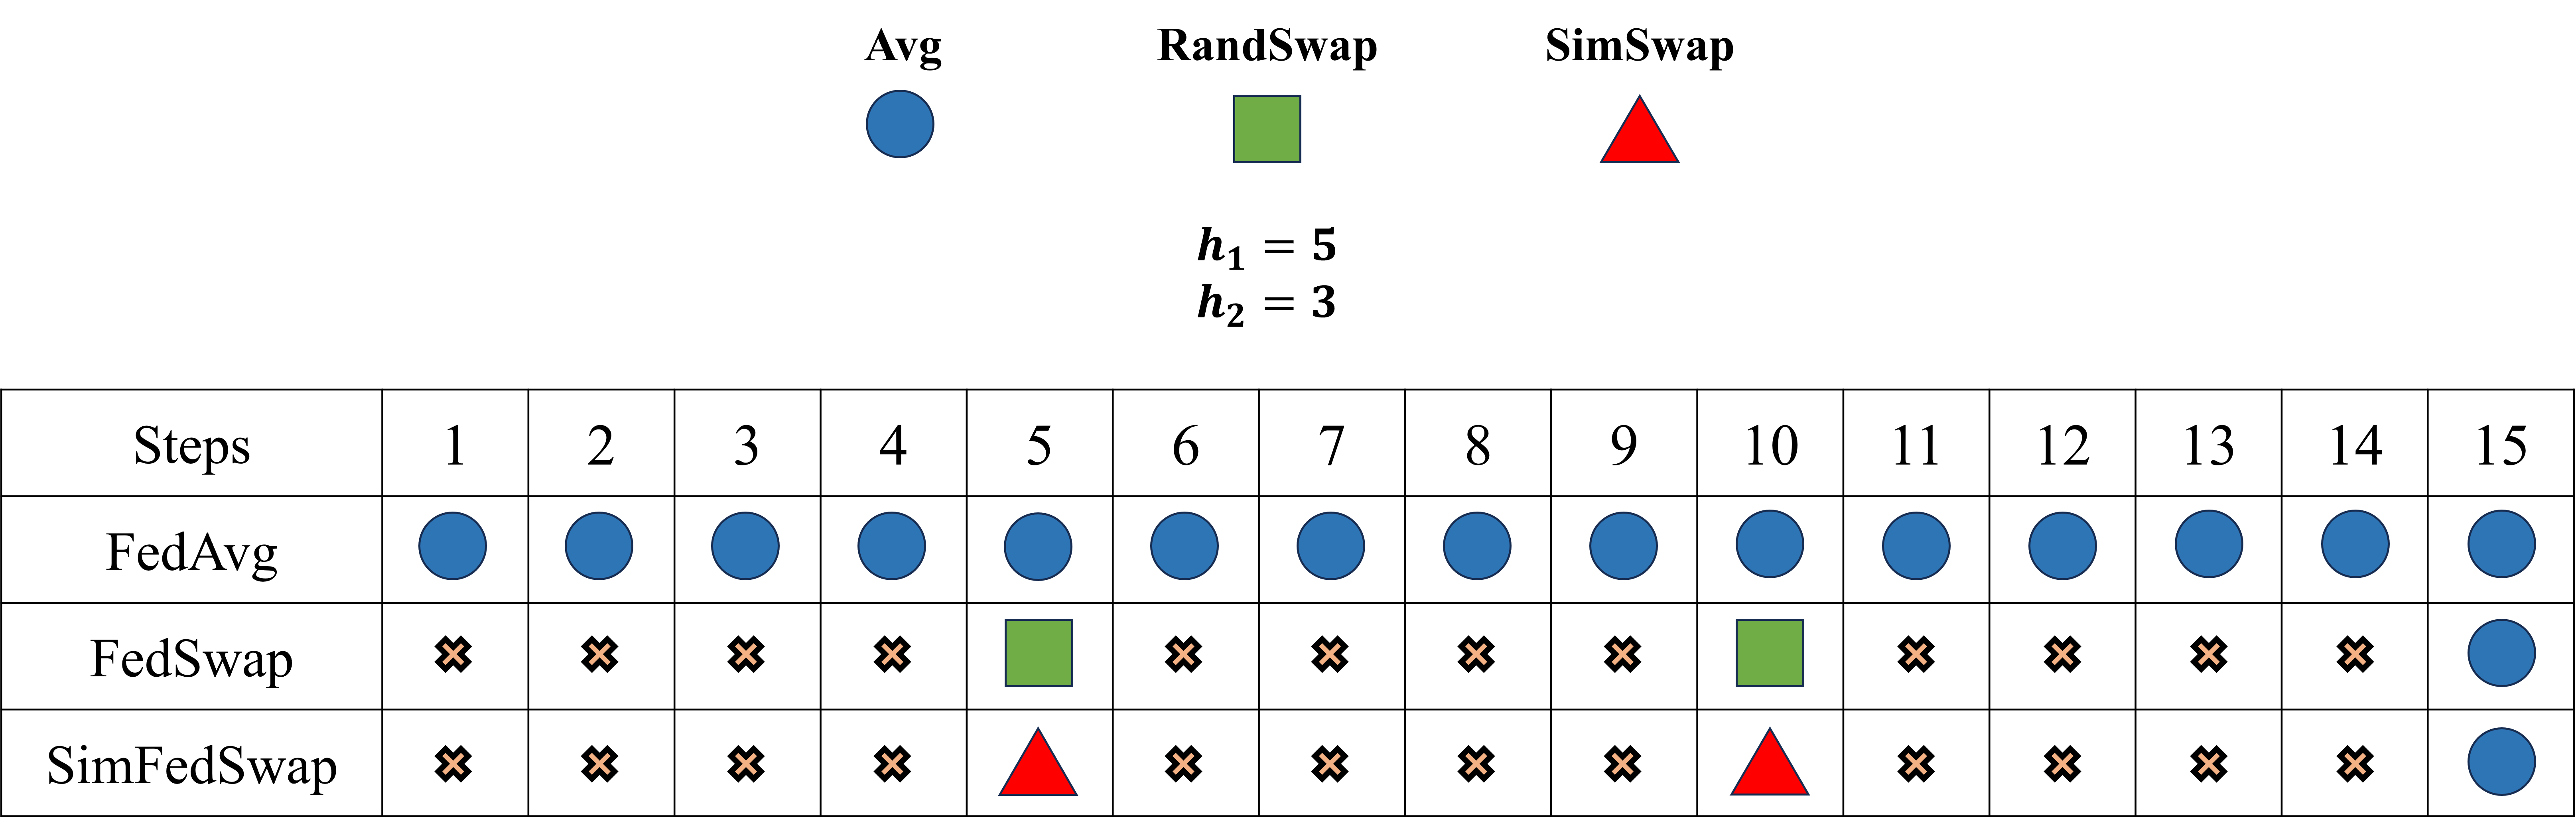
\includegraphics[scale=0.3]{images/chap4/compare_swap_net_traffic.png}%
	\caption{%
		تأثیر نحوه جابه‌جایی مدل‌ها بر ترافیک شبکه.
	}
	\label{compare_swap_net_traffic}
	\centering
\end{figure}
به‌طور خاص، در شبیه‌سازی‌هایی که پارامترهای \(h_1\) برابر با 5 و \(h_2\) برابر با 3 در نظر گرفته شده‌اند، روش \lr{FedSwap} موفق به کاهش
۸۶٫۶۶
درصدی هزینه‌های شبکه شده است. همچنین، روش \lr{SimFedSwap} توانسته این هزینه‌ها را تا ۸۰ درصد کاهش دهد. 


\subsubsection{
	تاثیر جابجایی مدل‌ها بر حریم شخصی در ارتباط بین سرور و کاربران
}
در روش یادگیری فدرال سنتی، مانند
\lr{FedAvg}%
، مدل‌ها پس از آموزش محلی توسط کاربران، به سرور مرکزی ارسال می‌شوند. سرور وظیفه تجمیع این مدل‌ها را بر عهده دارد و سپس مدل به‌روزرسانی‌ شده را به کاربران بازمی‌گرداند. در این روش، تعاملات فقط بین سرور و کاربران صورت می‌گیرد و هیچ ارتباط مستقیمی بین کاربران وجود ندارد. این امر باعث می‌شود که حریم شخصی کاربران به دلیل عدم تبادل مستقیم اطلاعات با یکدیگر، تا حد زیادی حفظ شود. همچنین کاربران نیازی به اعتماد به یکدیگر ندارند و تنها باید به سرور مرکزی اعتماد کنند.

در مقابل، در روش‌هایی که مدل‌ها بین خود کاربران جابه‌جا می‌شود، چه با واسطه سرور و چه بدون واسطه آن، خطرات بیشتری برای حریم شخصی وجود دارد. زمانی که مدل‌ها مستقیماً بین کاربران مبادله می‌شود، احتمال این که یکی از کاربران بتواند از طریق تحلیل مدل دریافت ‌شده اطلاعاتی در مورد داده‌های دیگر کاربران به دست آورد، افزایش می‌یابد. حتی اگر سرور به عنوان واسطه در این جابجایی‌ها عمل کند، همچنان خطراتی وجود خواهد داشت، زیرا سرور می‌تواند نقش ناظر را داشته باشد و از جابجایی مدل‌ها بین کاربران سوء استفاده کند. بنابراین، در هر دو حالت، جابجایی مدل‌ها بین کاربران نسبت به
\lr{FedAvg}
با چالش‌های بیشتری در زمینه حفظ حریم شخصی مواجه است.

در نتیجه، در روش
\lr{FedAvg}%
، به دلیل عدم ارتباط مستقیم بین کاربران، حریم شخصی به شکل بهتری حفظ می‌شود و تنها سرور مرکزی باید ایمن باشد. اما در روش جابجایی مدل‌ها بین کاربران، خطر نشت اطلاعات بین کاربران افزایش می‌یابد و این روش به پروتکل‌های امنیتی پیچیده‌تر و اعتماد بیشتر بین کاربران نیاز دارد.


\subsubsection{
	تاثیر جابجایی مدل‌ها بر حریم شخصی با توجه به واسطه بودن سرور
}
روش حریم خصوصی تفاضلی که در
\ref{privacy_challenge}
نیز به آن اشاره شد یکی از تکنیک‌های موثر برای حفظ حریم شخصی است که با اضافه کردن نویز به داده‌ها یا مدل‌ها، مانع از افشای اطلاعات حساس فردی می‌شود. این روش تضمین می‌کند که خروجی یک الگوریتم یادگیری به اندازه کافی تصادفی است، به‌طوری‌که حضور یا عدم حضور یک نمونه داده خاص در مجموعه داده‌ها، تاثیری بر خروجی نهایی نداشته باشد.

حال اگر از این روش در جابجایی مدل‌ها بین کاربران استفاده شود، تفاوت‌هایی بین دو رویکرد با واسطه سرور و بدون واسطه سرور وجود خواهد داشت. در حالتی که سرور واسطه باشد، اعمال حریم خصوصی تفاضلی می‌تواند به کنترل و مدیریت نویز اضافه شده کمک کند و سرور می‌تواند نقش فعالی در تضمین این که مدل‌ها به درستی ناشناس‌ شده‌اند، ایفا کند. این امر باعث می‌شود که خطر نشت اطلاعات به دلیل واسطه‌گری سرور کاهش یابد. اما همچنان باید به سرور اعتماد کرد که این فرآیند را به درستی انجام دهد.

در رویکرد بدون واسطه سرور، اعمال حریم خصوصی تفاضلی چالش‌برانگیزتر است، زیرا کاربران به‌طور مستقل باید نویز لازم را به مدل‌های خود اضافه کنند و در عین حال مطمئن شوند که سطح مناسبی از حفظ حریم شخصی برقرار است. در این حالت، هرگونه خطا یا ناهماهنگی در اعمال حریم خصوصی تفاضلی ممکن است منجر به افشای اطلاعات حساس شود. همچنین، نبود یک ناظر مرکزی مانند سرور، کار را برای هماهنگی و اجرای صحیح این روش پیچیده‌تر می‌کند.

در نتیجه، در صورت استفاده از روش حریم خصوصی تفاضلی، رویکرد با واسطه سرور به دلیل نظارت و کنترل متمرکز، از لحاظ حفظ حریم شخصی مزیت بیشتری دارد. در مقابل، در رویکرد بدون واسطه سرور، چالش‌های بیشتری برای کاربران وجود دارد که می‌تواند منجر به کاهش اثربخشی حریم خصوصی تفاضلی شود.
البته باید به این نکته اشاره کرد که حفظ حریم شخصی یکی از ارکان مهم در یادگیری فدرال است و برای سنجش دقیق میزان نفوذپذیری آن، لازم است روش‌های تخصصی در این حوزه به‌صورت مجزا پیاده‌سازی و بررسی شوند.
از آن جاکه در این پژوهش، تمرکز اصلی بر بهبود دقت مدل نهایی است، ورود به جزئیات حوزه امنیت خارج از محدوده مطالب مربوط به این پژوهش می‌باشد. با این حال تلاش شده تا حریم شخصی نیز تا حد امکان مورد توجه قرار گیرد.





\subsection{نحوه جابه‌جایی}
زمانی که همه مدل‌های شبکه عصبی در سرور مرکزی قرار دارند، وظیفه سرور این است که تصمیم بگیرد کدام کاربران مدل‌های خود را با یکدیگر جابه‌جا کنند. برای انجام این کار، ابتدا باید مدل‌ها با یکدیگر مقایسه شوند تا میزان شباهت بین آن‌ها مشخص شود. سپس، بر اساس این شباهت‌ها تعیین می‌شود که کدام کاربران مدل‌های شبکه عصبی خود را با یکدیگر مبادله کنند، یا به عبارت دیگر، سرور مشخص می‌کند کدام مدل به کدام کاربر ارسال شود.

\subsubsection{جابه‌جایی حریصانه}

در روش حریصانه، از بین تمام کاربران موجود، یک کاربر به‌صورت تصادفی انتخاب می‌شود. سپس مدل شبکه عصبی این کاربر با مدل‌های تمامی کاربران دیگر مقایسه می‌شود تا میزان شباهت آن‌ها سنجیده شود. در این مرحله، کاربری که مدل شبکه عصبی او کمترین شباهت را با مدل کاربر انتخاب‌ شده دارد، به عنوان کاربر مقصد برای جابه‌جایی مدل انتخاب می‌شود. پس از این انتخاب، سرور مدل‌های این دو کاربر را با یکدیگر جابه‌جا می‌کند و در نهایت این دو کاربر را از لیست انتخاب حذف خواهد کرد.

پس از انجام این جابه‌جایی، فرایند مشابهی برای کاربران باقی‌مانده تکرار می‌شود. ابتدا یک کاربر دیگر به‌صورت تصادفی انتخاب می‌شود و دقیقا همان روند بالا برای آن تکرار خواهد شد.
شبه کد کامل این روش در الگوریتم
\ref{algo_greedy_swapping}
ارائه شده است. علاوه بر این، نمادهای مختص به این الگوریتم در جدول
\ref{tabel_GreedySwappingNotations}
و همچنین تمامی نمادهای پایه در جدول
\ref{tabel_FedAvgNotations}
توضیح داده شده‌اند.
هدف از این جداول، فراهم کردن درکی جامع از نحوه عملکرد و پیاده‌سازی الگوریتم می‌باشد.


\begin{LTR}
	\SetAlgoNlRelativeSize{-1}
	\begin{algorithm}[t]
		\begin{RTL}
			\caption{%
				جابه‌جایی حریصانه
				\lr{(Greedy Swapping)}
			}
			\label{algo_greedy_swapping}
		\end{RTL}
		
		\begin{latin}
			\SetKwFunction{GreedySwapping}{GreedySwapping}
			\SetKwProg{Fn}{Function}{:}{end}
			\Fn{\GreedySwapping{}}{
				$LRS$ = copy of $U_t$\;
				$NS$ = (length of $U_t$ // 2) * $SP$\;
				\BlankLine
				
				\For{$NS$ times}{
					$RandomIndex$ = random integer between $0$ and length of $LRS$\;
					$SCB = LRS[RandomIndex]$\;
					remove $SCB$ from $LRS$\;
					
					\BlankLine
					Initialize $LstSimilarity$ as an empty list\;
					\For{each $RC \in LRS$}{
						$Sim = \texttt{ModelSimilarity} (w^{SCB}, w^{RC})$\;
						Append $Sim$ to $LstSimilarity$\;
					}
					$MinSimilarityIndex$ = index of the minimum value in $LstSimilarity$\;
					$SCD = LRS[MinSimilarityIndex]$\;
					remove $SCD$ from $LRS$\;
					\BlankLine
					
					$\texttt{Swap}(SCB, SCD)$\;
				}
			}
		\end{latin}
	\end{algorithm}
\end{LTR}

\begin{table}[h]
	\centering
	\caption{نمادهای مختص الگوریتم جابه‌جایی حریصانه}
	\label{tabel_GreedySwappingNotations}
	\begin{tabular}{cr}
		\hline
		متغیر & توضیحات \\
		\hline
		$LRS \, (LstRemainSwap)$ & لیست باقی‌مانده جابه‌جایی \\
		$NS \, (NumSwaps)$ & تعداد جابه‌جایی‌ها \\
		$SP \, (SwapPercentage)$ & ضریب کنترلی برای تعداد جابه‌جایی‌ها \\
		$RandomIndex$ & شاخص تصادفی \\
		$SCB \, (SwapClientBase)$ & کاربر مبدا جابه‌جایی \\
		$LstSimilarity$ & لیست مشابهت \\
		$RC \, (RemainClient)$ & کاربر باقی‌مانده \\
		$Sim$ & معیار مشابهت بین دو مدل شبکه عصبی \\
		$SCD \, (SwapClientDest)$ & کاربر مقصد جابه‌جایی
	\end{tabular}
\end{table}




\subsubsection{جابه‌جایی حداقل شباهت}

در این روش، برای این که حداقل شباهت ممکن بین تمامی مدل‌های شبکه عصبی به دست آید، لازم است تمامی مدل‌ها با یکدیگر مقایسه شوند و دو مدلی که کمترین شباهت را دارند با هم جابه‌جا شوند. به عنوان مثال، اگر \( n \) مدل وجود داشته باشد، باید یک ماتریس \( n \times n \) برای بررسی میزان شباهت‌ها ایجاد شود. در این ماتریس، شباهت مدل 1 با مدل 2 برابر با شباهت مدل 2 با مدل 1 در نظر گرفته می‌شود. همچنین به دلیل این که مقایسه یک مدل با خودش بی‌معنی است، ماتریس نهایی به شکل یک ماتریس بالا مثلثی%
\LTRfootnote{Upper Triangular Matrix}
(بدون قطر اصلی) تبدیل می‌شود. به این صورت که تنها حدود نیمی از ماتریس، شامل شباهت‌های مورد نیاز برای مقایسه است. در نتیجه ماتریس مورد نظر به شکل زیر در خواهد آمد.
\begin{equation}
	\begin{bmatrix}
		\infty & a^{12} & a^{13} & \cdots & a^{1n} \\
		\infty & \infty & a^{23} & \cdots & a^{2n} \\
		\infty & \infty & \infty & \cdots & a^{3n} \\
		\vdots & \vdots & \vdots & \ddots & \vdots \\
		\infty & \infty & \infty & \cdots & \infty
	\end{bmatrix}
	\label{eq_similarity_matrix}
\end{equation}

ابتدا، تمامی شباهت‌ها بین مدل‌ها محاسبه می‌شود و سپس از ماتریس ایجاد شده، کمترین مقدار شباهت انتخاب می‌شود. شماره سطر و ستون متناظر با این مقدار نشان می‌دهد که این دو مدل باید با یکدیگر جابه‌جا شوند. پس از انجام این جابه‌جایی، تمامی مقدارهای مربوط به سطر و ستون متناظر با این دو مدل باید به بی‌نهایت تغییر داده شوند تا در مراحل بعدی مجدد انتخاب نشوند. همچنین باید دقت کرد که هر دو سطر و ستون مرتبط با این دو مدل باید به بی‌نهایت تغییر داده شوند.

برای درک بهتر، فرض کنید کمترین مقدار شباهت در سطر سوم و ستون ششم ماتریس قرار دارد. در این حالت، مدل‌های سوم و ششم باید با یکدیگر جابه‌جا شوند. پس از این جابه‌جایی، لازم است که تمامی مقادیر در سطرهای سوم و ششم و همچنین ستون‌های سوم و ششم به بی‌نهایت تغییر کنند تا این دو مدل دیگر مورد بررسی قرار نگیرند. به این ترتیب، در دور بعدی، کوچک‌ترین مقدار شباهت از ماتریس انتخاب می‌شود و چون مقادیر مربوط به مدل‌های سوم و ششم به بی‌نهایت تغییر کرده‌اند، دیگر در این مرحله حضور نخواهند داشت و انتخاب نمی‌شوند. شبه کد کامل این روش در الگوریتم
\ref{algo_min_similarity_swapping}
ارائه شده است. علاوه بر این، نمادهای مختص به این الگوریتم در جدول
\ref{tabel_MinSimilaritySwapNotations}
توضیح داده شده‌اند.


\begin{LTR}
	\SetAlgoNlRelativeSize{-1}
	\begin{algorithm}[t]
		\begin{RTL}
			\caption{%
				جابه‌جایی حداقل شباهت
				\lr{(Minimum Similarity Swapping)}
			}
			\label{algo_min_similarity_swapping}
		\end{RTL}
		
		\begin{latin}
			\SetKwFunction{MinSimilaritySwapping}{MinSimilaritySwapping}
			\SetKwProg{Fn}{Function}{:}{end}
			\Fn{\MinSimilaritySwapping{}}{
				Initialize $SimArray$\;
				$L$ = length of $U_t$\;
				\BlankLine
				
				\For{each $row$ from $0$ to $L$}{
					\For{each $col$ from $(row+1)$ to $L$}{
						$Sim = \texttt{ModelSimilarity} (w^{row}, w^{col})$\;
						Append $Sim$ to $SimArray$\;
					}
				}
				\BlankLine
				
				$NS$ = ($L$ // 2) * $SP$\;
				\For{$NS$ times}{
					$MI$ = index of minimum value in $SimArray$\;
					$row, col$ = find $row$ and $col$ number, based on $MI$\;					
					Set all values of $SimArray[row, col]$ to $\infty$\;
					\BlankLine
					
					$\texttt{Swap}(w^{row}, w^{col})$\;
				}
			}
		\end{latin}
	\end{algorithm}
\end{LTR}


\begin{table}[h]
	\centering
	\caption{نمادهای مختص الگوریتم جابه‌جایی حداقل شباهت}
	\label{tabel_MinSimilaritySwapNotations}
	\begin{tabular}{cr}
		\hline
		متغیر & توضیحات \\
		\hline
		$SimArray$ & آرایه مشابهت \\
		$L$ & طول مجموعه‌ای از کاربران در گام $t$ \\
		$MI \, (MinIndex)$ & شاخص مقدار کمینه در آرایه مشابهت \\
		$row$ & شماره سطر بر اساس دید ماتریس مشابهت \\
		$col$ & شماره ستون بر اساس دید ماتریس مشابهت
	\end{tabular}
\end{table}








\section{بررسی نتایج}
\subsection{
	مجموعه داده
	\lr{\texttt{\fontspec{Times New Roman} MNIST}}%
	\LTRfootnote{Modified National Institute of Standards and Technology}
}
اکنون نتایج مربوط به مجموعه داده
\lr{MNIST}
بررسی خواهد شد که شکل
\ref{result_mnist_mlp}
نتایج مقایسه روش
\lr{SimFedSwap}
با سایر روش‌های مرجع را با استفاده از مدل
\lr{MLP}
به تصویر می‌کشد.
\begin{figure}[t]
	\centering
	\subfigure[
	دید کلی از نتیجه
	\qquad\hspace{3mm}]{
		\label{result_mnist_mlp_mid}
		\includegraphics*[width=.441\textwidth]{images/chap5/result/mnist/acc_mid_mlp.png}
	}
	\hspace{0.8mm}
	\subfigure[
	بزرگ‌نمایی شده بخش اصلی					
	\qquad\hspace{5mm}]{
		\label{result_mnist_mlp_zoom}
		\includegraphics*[width=.441\textwidth]{images/chap5/result/mnist/acc_zoom_mlp.png}
	}
	\caption{
		مقایسه منحنی‌های دقت در مجموعه داده
		\lr{MNIST}
		با استفاده از مدل
		\lr{MLP}.
	}
	\label{result_mnist_mlp}
\end{figure}
همچنین، پارامترهای به‌کاررفته در این اجرا در جدول
\ref{tabel_parameter_mnist} 
به نمایش درآمده‌اند.
%\addtolength{\tabcolsep}{-0.5mm}
\begin{table}[t]
	\centering
	\caption{
		پارامترهای اجرا در مجموعه داده
		\lr{MNIST}
	}
	\label{tabel_parameter_mnist}
	%	\scalebox{0.985}{
		\begin{tabular}{ccccccccccccc}
			\hline
			\specialcell{مجموعه\\داده} &
			\specialcell{نحوه\\جابه‌جایی} &
			\specialcell{توزیع\\داده} &
			$K$ &
			$B$ &
			$C$ &
			$SP$ &
			$\eta$ &
			$E$ &
			$h_1$ &
			$h_2$
			\\
			\hline
			\lr{MNIST} &
			\lr{MSS} &
			نرمال &
			\lr{10} &
			\lr{32} &
			\lr{1.0} &
			\lr{1.0} &
			\lr{0.001} &
			\lr{1} &
			\lr{5} &
			\lr{3}
			\\
		\end{tabular}
		%	}
\end{table}
نکته قابل توجه این است که منحنی‌های
\lr{FedAvg} 
و
\lr{FedSwap} 
به عنوان منحنی‌های نهایی و مرجع بر روی سایر منحنی‌ها قرار گرفته‌اند. در صورتی که رنگ متفاوتی در نمودار دیده شود، این موضوع نشان‌دهنده اختلاف عملکرد روش مربوطه در آن نقطه خواهد بود. این تغییر ممکن است نشان‌دهنده عملکرد بهتر یا ضعیف‌تر در مقایسه با دیگر روش‌ها باشد و می‌تواند به عنوان مبنایی برای مقایسه و تحلیل مورد توجه قرار گیرد.




همان‌طور که در شکل
\ref{result_mnist_mlp} 
مشاهده می‌شود، روش‌های مبتنی‌بر جابه‌جایی به شکل بسیار ناچیزی از روش
\lr{FedAvg} 
نتایج مطلوب‌تری را ارائه داده‌اند. نکته قابل توجه این است که همه روش‌های مبتنی‌بر جابه‌جایی عملکردی مشابه داشته‌اند. برای بررسی دقیق‌تر این اجرا، منحنی‌های خطا در شکل
\ref{app_result_mnist_mlp}
پیوست، قابل مشاهده هستند.


در شکل
\ref{result_mnist_cnn}
همان آزمایش قبلی تکرار شده، با این تفاوت که این مرتبه از مدل شبکه عصبی
\lr{CNN}
استفاده شده است. همان‌طور که دیده می‌شود، تقریباً تمامی روش‌ها عملکرد مشابهی داشته‌اند. این نکته نشان می‌دهد که وقتی شبکه به راحتی به دقت بالایی می‌رسد، تفاوتی در نتایج بین روش‌ها دیده نمی‌شود. برای جزئیات بیشتر این اجرا، منحنی‌های خطا در شکل
\ref{app_result_mnist_cnn}
پیوست، آمده‌اند.


\begin{figure}[t]
	\centering
	\subfigure[
	دید کلی از نتیجه
	\qquad\hspace{3mm}]{
		\label{result_mnist_cnn_mid}
		\includegraphics*[width=.48\textwidth]{images/chap5/result/mnist/acc_mid_cnn.png}
	}
	\hspace{0.8mm}
	\subfigure[
	بزرگ‌نمایی شده بخش اصلی					
	\qquad\hspace{5mm}]{
		\label{result_mnist_cnn_zoom}
		\includegraphics*[width=.48\textwidth]{images/chap5/result/mnist/acc_zoom_cnn.png}
	}
	\caption{
		مقایسه منحنی‌های دقت در مجموعه داده
		\lr{MNIST}
		با استفاده از مدل
		\lr{CNN}.
	}
	\label{result_mnist_cnn}
\end{figure}





\FloatBarrier
\subsection{
	مجموعه داده
	\lr{\texttt{\fontspec{Times New Roman} CIFAR-10}}%
	\LTRfootnote{Canadian Institute For Advanced Research}
}
اکنون نتایج مربوط به مجموعه داده
\lr{CIFAR-10}
بررسی خواهد شد که شکل
\ref{result_cifar10_equal}
نتایج مقایسه روش
\lr{SimFedSwap}
با سایر روش‌های مرجع را با توزیع داده یکنواخت بین کاربران به تصویر می‌کشد.
پارامترهای استفاده شده در این آزمایش نیز در جدول
\ref{tabel_parameter_cifar10}
به نمایش درآمده‌اند.


\begin{figure}[t]
	\centering
	\subfigure[
	دید کلی از نتیجه
	\qquad\hspace{3mm}]{
		\label{result_cifar10_equal_mid}
		\includegraphics*[width=.48\textwidth]{images/chap5/result/cifar10/acc_mid_equal.png}
	}
	\hspace{0.8mm}
	\subfigure[
	بزرگ‌نمایی شده بخش اصلی					
	\qquad\hspace{5mm}]{
		\label{result_cifar10_equal_zoom}
		\includegraphics*[width=.48\textwidth]{images/chap5/result/cifar10/acc_zoom_equal.png}
	}
	\caption{
		مقایسه منحنی‌های دقت در مجموعه داده
		\lr{CIFAR-10}
		با توزیع داده یکنواخت.
	}
	\label{result_cifar10_equal}
\end{figure}


%\addtolength{\tabcolsep}{-0.5mm}
\begin{table}[t]
	\centering
	\caption{
		پارامترهای اجرا در مجموعه داده
		\lr{CIFAR-10}
	}
	\label{tabel_parameter_cifar10}
	%	\scalebox{0.985}{
		\begin{tabular}{ccccccccccccc}
			\hline
			\specialcell{مجموعه\\داده} &
			\specialcell{شبکه\\عصبی} &
			\specialcell{نحوه\\جابه‌جایی} &
			$K$ &
			$B$ &
			$C$ &
			$SP$ &
			$\eta$ &
			$E$ &
			$h_1$ &
			$h_2$
			\\
			\hline
			\lr{CIFAR-10} &
			\lr{Conv} &
			\lr{MSS} &
			\lr{10} &
			\lr{64} &
			\lr{1.0} &
			\lr{1.0} &
			\lr{0.001} &
			\lr{2} &
			\lr{3} &
			\lr{10}
			\\
		\end{tabular}
		%	}
\end{table}


همان‌طور که در شکل
\ref{result_cifar10_equal}
مشاهده می‌شود، روش‌های مبتنی‌بر جابه‌جایی نسبت به روش
\lr{FedAvg}
عملکرد متمایزی داشته‌اند. با این حال، این روش‌ها در یک سطح عملکردی نزدیک به هم قرار گرفته‌اند. به‌طور کلی، با وجود اختلافات جزئی، روش‌های مبتنی‌بر شباهت در مقایسه با روش
\lr{FedSwap}
کمی بهتر عمل کرده‌اند. برای آگاهی از جزئیات بیشتر، به منحنی‌های خطا در شکل
\ref{app_result_cifar10_equal}
پیوست، توجه نمایید.


در شکل
\ref{result_cifar10_normal}%
، آزمایش قبلی دوباره اجرا شده، اما این بار از توزیع داده نرمال استفاده شده است. مشاهده می‌شود که در این وضعیت نیز روش‌های مبتنی‌بر جابه‌جایی، عملکرد بهتری نسبت به روش
\lr{FedAvg}
داشته‌اند. البته، نتایج حاصل از روش‌های جابه‌جایی تقریباً مشابه بوده و تفاوت قابل توجهی بین آن‌ها دیده نمی‌شود. برای مشاهده جزئیات بیشتر، می‌توان به منحنی‌های خطا در شکل
\ref{app_result_cifar10_normal}
پیوست، مراجعه کرد.

\begin{figure}[t]
	\centering
	\subfigure[
	دید کلی از نتیجه
	\qquad\hspace{3mm}]{
		\label{result_cifar10_normal_base}
		\includegraphics*[width=.48\textwidth]{images/chap5/result/cifar10/acc_base_normal.png}
	}
	\hspace{0.8mm}
	\subfigure[
	بزرگ‌نمایی شده بخش اصلی					
	\qquad\hspace{5mm}]{
		\label{result_cifar10_normal_zoom}
		\includegraphics*[width=.48\textwidth]{images/chap5/result/cifar10/acc_zoom_normal.png}
	}
	\caption{
		مقایسه منحنی‌های دقت در مجموعه داده
		\lr{CIFAR-10}
		با توزیع داده نرمال.
	}
	\label{result_cifar10_normal}
\end{figure}




\FloatBarrier
\subsection{
	مجموعه داده
	\lr{\texttt{\fontspec{Times New Roman} CINIC-10}}%
	\LTRfootnote{CIFAR-10 and ImageNet Combined}
}

اکنون نتایج مربوط به مجموعه داده
\lr{CINIC-10}
بررسی خواهد شد که شکل
\ref{result_cinic10}
نتایج مقایسه روش
\lr{SimFedSwap}
با سایر روش‌های مرجع را به تصویر می‌کشد.
همچنین، پارامترهای به کار رفته در این آزمایش در جدول
\ref{tabel_parameter_cinic10}
ارائه شده‌اند.

\begin{figure}[t]
	\centering
	\subfigure[
	دید کلی از نتیجه
	\qquad\hspace{3mm}]{
		\label{result_cinic10_mid}
		\includegraphics*[width=.48\textwidth]{images/chap5/result/cinic10/acc_mid.png}
	}
	\hspace{0.8mm}
	\subfigure[
	بزرگ‌نمایی شده بخش اصلی					
	\qquad\hspace{5mm}]{
		\label{result_cinic10_zoom}
		\includegraphics*[width=.48\textwidth]{images/chap5/result/cinic10/acc_zoom.png}
	}
	\caption{
		مقایسه منحنی‌های دقت در مجموعه داده
		\lr{CINIC-10}.
	}
	\label{result_cinic10}
\end{figure}


%\addtolength{\tabcolsep}{-0.5mm}
\begin{table}[t]
	\centering
	\caption{
		پارامترهای اجرا در مجموعه داده
		\lr{CINIC-10}
	}
	\label{tabel_parameter_cinic10}
	%	\scalebox{0.985}{
		\begin{tabular}{ccccccccccccc}
			\hline
			\specialcell{مجموعه\\داده} &
			\specialcell{شبکه\\عصبی} &
			\specialcell{نحوه\\جابه‌جایی} &
			\specialcell{توزیع\\داده} &
			$K$ &
			$B$ &
			$C$ &
			$SP$ &
			$\eta$ &
			$E$ &
			$h_1$ &
			$h_2$
			\\
			\hline
			\lr{CINIC-10} &
			\lr{Conv} &
			\lr{MSS} &
			نرمال &
			\lr{30} &
			\lr{64} &
			\lr{0.5} &
			\lr{1.0} &
			\lr{0.001} &
			\lr{1} &
			\lr{2} &
			\lr{5}
			\\
		\end{tabular}
		%	}
\end{table}


در شکل
\ref{result_cinic10}
به‌وضوح می‌توان مشاهده کرد که روش‌های مبتنی‌بر جابه‌جایی در مقایسه با روش
\lr{FedAvg}%
، عملکرد متفاوتی داشته‌اند. هرچند، این روش‌ها همچنان در یک سطح عملکردی نزدیک به هم قرار دارند و تفاوت‌های عمده‌ای میان آن‌ها دیده نمی‌شود. برای بررسی دقیق‌تر، منحنی‌های خطا در شکل
\ref{app_result_cinic10}
پیوست، به تفصیل آمده‌اند.







\FloatBarrier
\subsection{
	مجموعه داده
	\lr{\texttt{\fontspec{Times New Roman} FEMNIST}}%
	\LTRfootnote{Federated Extended MNIST}
}
در این مجموعه داده، تعداد داده‌ها در هر کلاس یکسان نیست و کلاس‌های مختلف دارای تعداد متفاوتی از داده‌ها هستند. شکل
\ref{count_all_classes}%
، تعداد داده‌های هر کلاس و نحوه نام‌گذاری آن‌ها را نشان می‌دهد.


\begin{figure}[t]
	\centering
	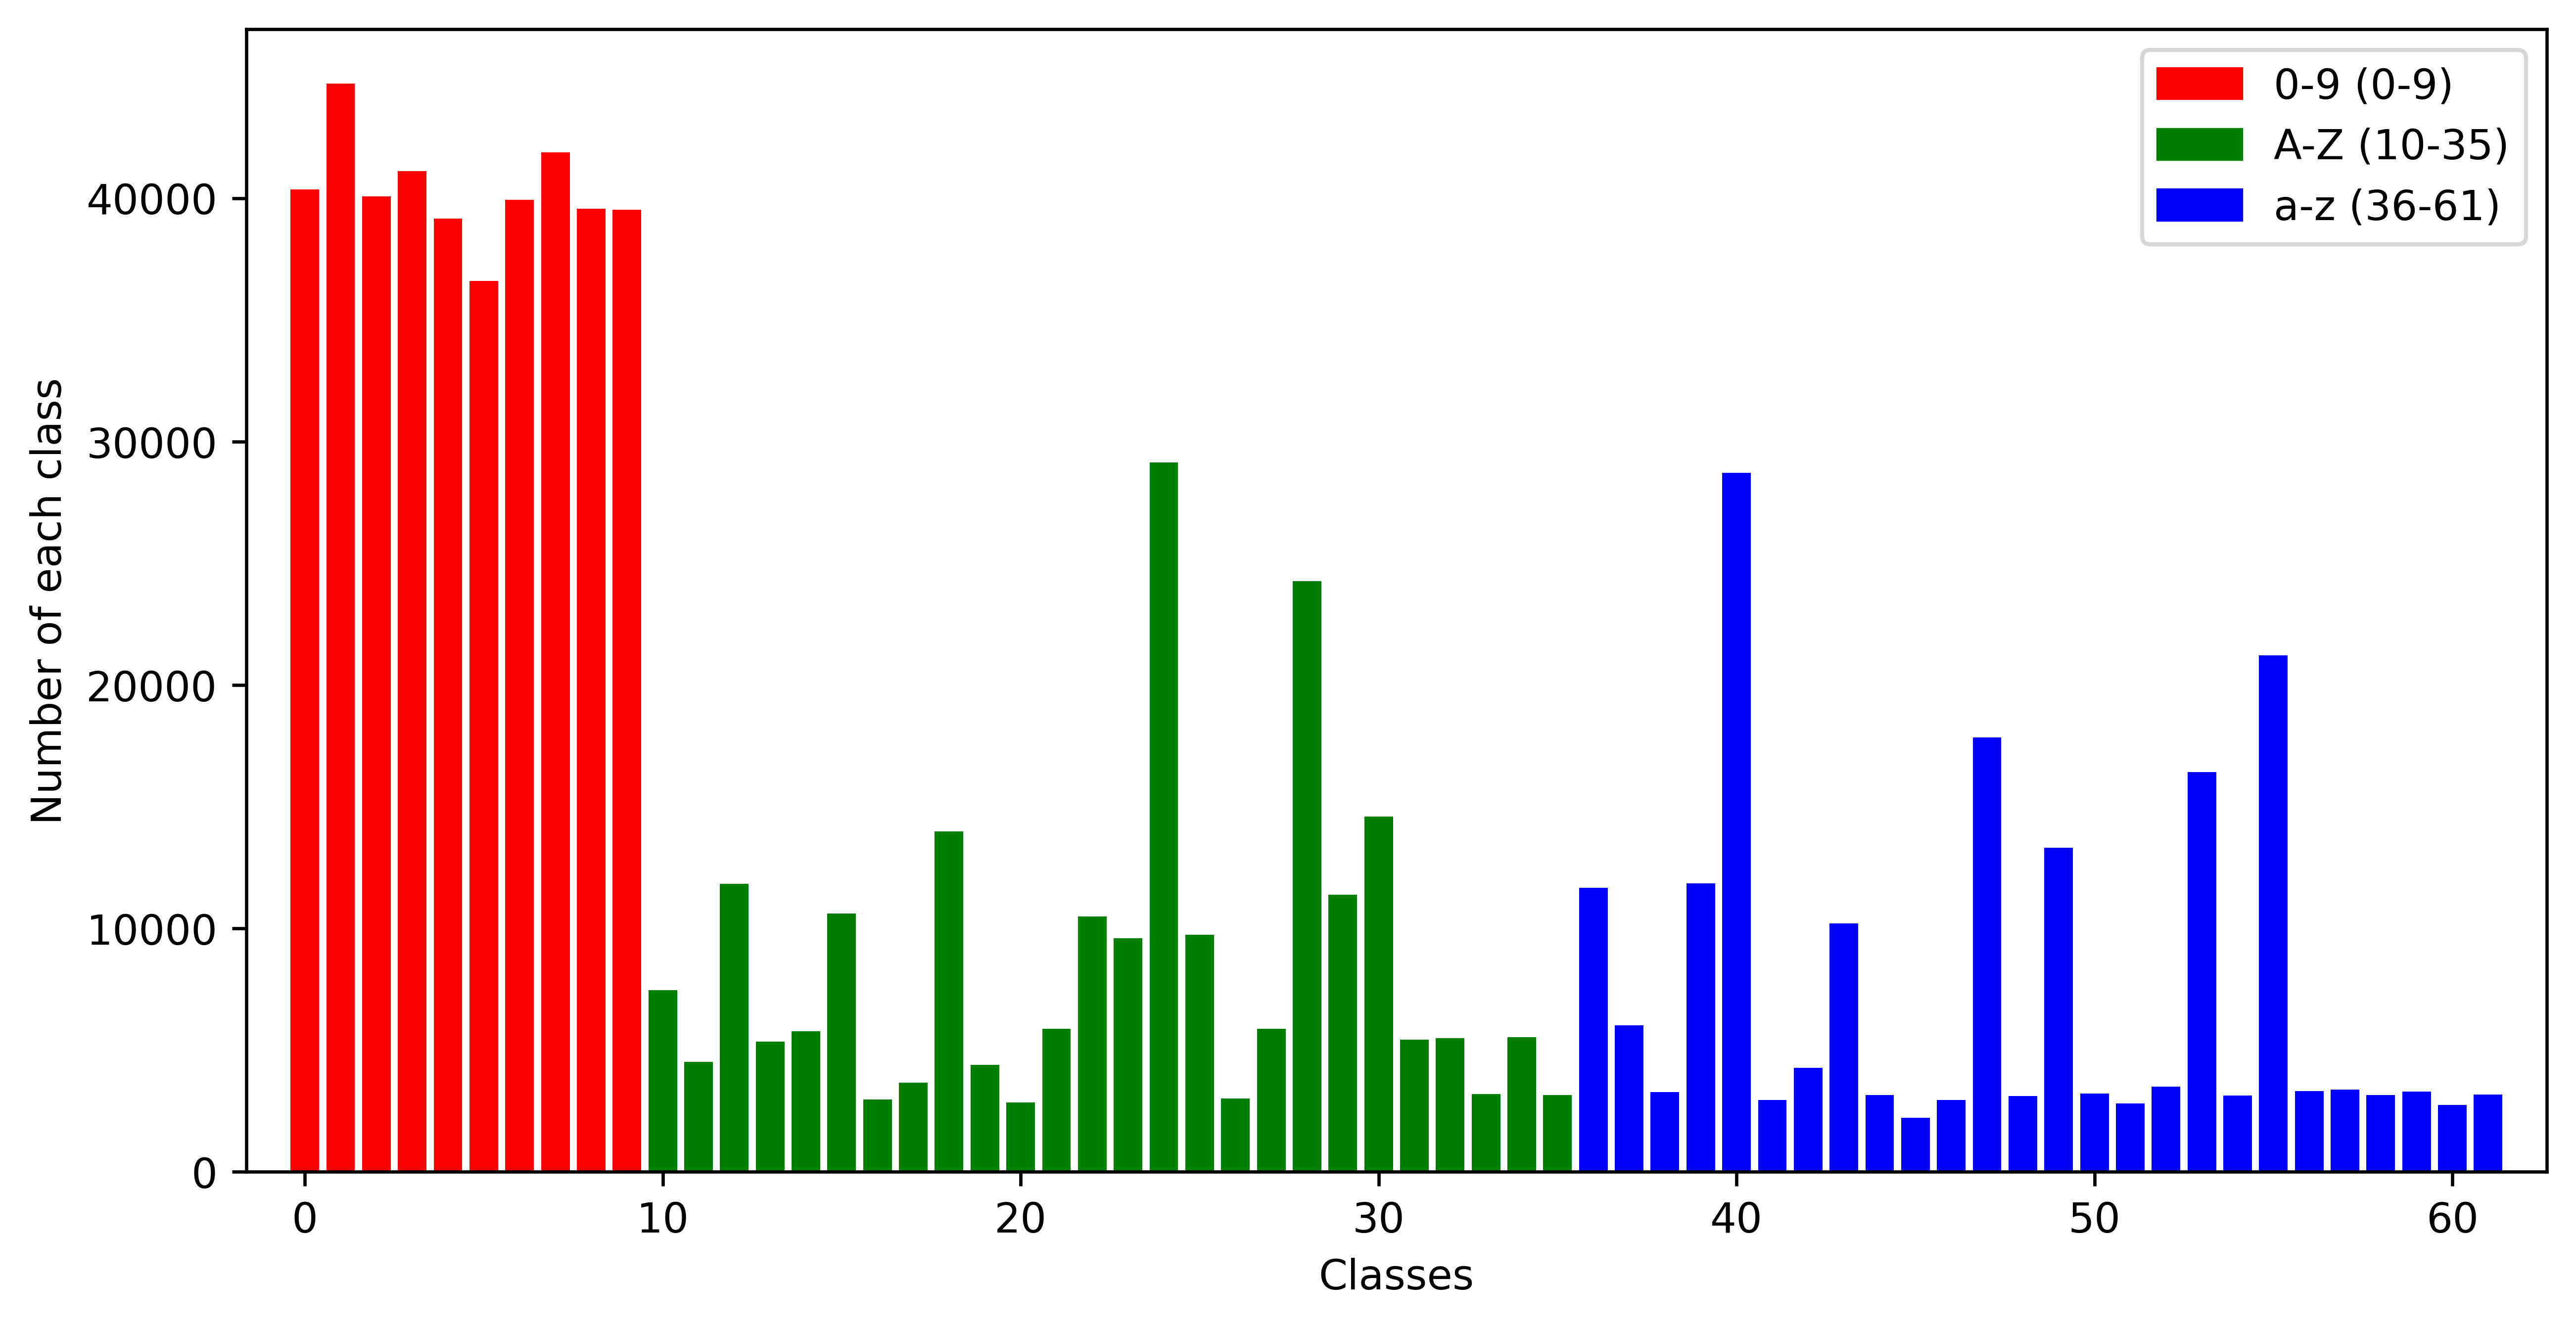
\includegraphics[scale=0.7]{images/chap5/count_all_classes.png}%
	\caption{%
		تعداد داده‌های هر کلاس و نحوه نام‌گذاری در مجموعه داده
		\lr{FEMNIST}.
	}
	\label{count_all_classes}
	\centering
\end{figure}

همان‌طور که در شکل
\ref{count_all_classes}
مشاهده می‌شود، تعداد کلاس‌های 0 تا 9 که به ارقام 0 تا 9 اشاره دارند، به‌طور قابل‌توجهی بیشتر از سایر کلاس‌هاست و هر کدام حدود 40٬000 نمونه دارند. در بین کلاس‌های 10 تا 35 که مربوط به حروف بزرگ انگلیسی هستند، کلاس‌های \lr{S} و \lr{O} بیشترین تعداد نمونه را دارند. به نظر می‌رسد این سبک از جمع‌آوری داده به دلیل جلوگیری از اشتباه گرفتن کلاس \lr{O} با عدد صفر و کلاس \lr{S} با معادل حرف کوچک آن در کلاس‌های 36 تا 61 بوده باشد.


مجموعه داده
\lr{FEMNIST}
به‌صورت پیش‌فرض شامل 3597 کاربر است که داده‌ها میان این کاربران توزیع شده‌اند. این توزیع، نه از لحاظ تعداد تصاویر بین کاربران و نه از لحاظ پوشش‌دهی کلاس‌ها در هر کاربر، یکسان نیست. با این حال، تعداد کاربران و نحوه توزیع داده‌ها میان آن‌ها را می‌توان به دلخواه تغییر داد.



اکنون رویکردهای پایه در مجموعه داده
\lr{FEMNIST}
بررسی خواهند شد. در رویکرد اول، داده‌ها بدون توجه به کاربران اصلی و تنها بر اساس کلاس‌های آن‌ها تفکیک می‌شوند. به این صورت که تمام داده‌های مربوط به هر کلاس جمع‌آوری شده و طبق یک توزیع مشخص بین تعدادی کاربر تقسیم می‌شوند. این روش به عنوان رویکرد کلاس‌بندی یا
\lr{FEMNISTclass}
شناخته می‌شود.

در رویکرد دوم، ساختار اصلی مجموعه داده تغییر نمی‌کند و تعداد کاربران همان تعداد پیش‌فرض باقی می‌ماند. همچنین داده‌ها دقیقا به همان شیوه‌ای که به هر کاربر اختصاص داده شده‌اند، حفظ می‌شوند. این روش به نام رویکرد نویسندگان یا
\lr{FEMNISTwriter}
نام‌گذاری شده است. در ادامه نتایج مربوط به هر کدام از این رویکرد‌ها به‌صورت مجزا بررسی خواهد شد.






\subsubsection{
	مقایسه نتایج در رویکرد کلاس‌بندی
	\lr{\texttt{\fontspec{Times New Roman} (FEMNISTclass)}}
}

نتایج مقایسه روش
\lr{SimFedSwap}
با دیگر روش‌های مرجع در شکل
\ref{result_FEMNISTclass}
نمایش داده شده‌اند که این آزمایش بر روی مجموعه داده
\lr{FEMNISTclass}
انجام شده است. پارامترهای مورد استفاده در این آزمایش نیز در جدول
\ref{tabel_parameter_FEMNISTclass}
ذکر شده‌اند.


\begin{figure}[t]
	\centering
	\subfigure[
	دید کلی از نتیجه
	\qquad\hspace{3mm}]{
		\label{result_FEMNISTclass_base}
		\includegraphics*[width=.48\textwidth]{images/chap5/result/FEMNISTclass/acc_base.png}
	}
	\hspace{0.8mm}
	\subfigure[
	بزرگ‌نمایی شده بخش اصلی					
	\qquad\hspace{5mm}]{
		\label{result_FEMNISTclass_zoom}
		\includegraphics*[width=.48\textwidth]{images/chap5/result/FEMNISTclass/acc_zoom.png}
	}
	\caption{
		مقایسه منحنی‌های دقت در مجموعه داده
		\lr{FEMNISTclass}.
	}
	\label{result_FEMNISTclass}
\end{figure}


%\addtolength{\tabcolsep}{-0.5mm}
\begin{table}[t]
	\centering
	\caption{
		پارامترهای اجرا در مجموعه داده
		\lr{FEMNISTclass}
	}
	\label{tabel_parameter_FEMNISTclass}
	%	\scalebox{0.985}{
		\begin{tabular}{ccccccccccccc}
			\hline
			\specialcell{مجموعه\\داده} &
			\specialcell{شبکه\\عصبی} &
			\specialcell{نحوه\\جابه‌جایی} &
			\specialcell{توزیع\\داده} &
			$K$ &
			$B$ &
			$C$ &
			$SP$ &
			$\eta$ &
			$E$ &
			$h_1$ &
			$h_2$
			\\
			\hline
			\lr{FEMNISTclass} &
			\lr{Conv} &
			\lr{MSS} &
			یکنواخت &
			\lr{200} &
			\lr{1024} &
			\lr{1.0} &
			\lr{1.0} &
			\lr{0.001} &
			\lr{2} &
			\lr{5} &
			\lr{3}
			\\
		\end{tabular}
		%	}
\end{table}



از شکل
\ref{result_FEMNISTclass}
مشخص است که روش‌های مبتنی‌بر جابه‌جایی در مقایسه با
\lr{FedAvg}
عملکرد متفاوتی نشان می‌دهند، اما همچنان تفاوت‌های عملکردی بین آن‌ها محدود و نزدیک به هم است.
نکته قابل توجه این است که بسیاری از تغییرات در نمودارها به لحظات جابه‌جایی یا میانگین‌گیری مربوط می‌شوند.
برای جزئیات بیشتر و بررسی دقیق‌تر، می‌توان به منحنی‌های خطا که در شکل
\ref{app_result_FEMNISTclass}
پیوست آمده‌اند، مراجعه کرد.




\subsubsection{
	مقایسه نتایج در رویکرد نویسندگان
	\lr{\texttt{\fontspec{Times New Roman} (FEMNISTwriter)}}
}
نتایج مربوط به مقایسه روش
\lr{SimFedSwap}
با سایر روش‌های مرجع در شکل
\ref{result_FEMNISTwriter_one}
قابل مشاهده است. این آزمایش بر روی مجموعه داده
\lr{FEMNISTwriter}
اجرا شده و پارامترهای به‌کاررفته در آن نیز در جدول
\ref{tabel_parameter_FEMNISTwriter}
ذکر شده‌اند.


\begin{figure}[t]
	\centering
	\subfigure[
	دید کلی از نتیجه
	\qquad\hspace{3mm}]{
		\label{result_FEMNISTwriter_one_base}
		\includegraphics*[width=.48\textwidth]{images/chap5/result/FEMNISTwriter/acc_base_one.png}
	}
	\hspace{0.8mm}
	\subfigure[
	بزرگ‌نمایی شده بخش اصلی					
	\qquad\hspace{5mm}]{
		\label{result_FEMNISTwriter_one_zoom}
		\includegraphics*[width=.48\textwidth]{images/chap5/result/FEMNISTwriter/acc_zoom_one.png}
	}
	\caption{
		مقایسه منحنی‌های دقت در یک اجرا بر روی مجموعه داده
		\lr{FEMNISTwriter}.
	}
	\label{result_FEMNISTwriter_one}
\end{figure}


%\addtolength{\tabcolsep}{-0.5mm}
\begin{table}[t]
	\centering
	\caption{
		پارامترهای اجرا در مجموعه داده
		\lr{FEMNISTwriter}
	}
	\label{tabel_parameter_FEMNISTwriter}
	%	\scalebox{0.985}{
		\begin{tabular}{ccccccccccccc}
			\hline
			\specialcell{مجموعه\\داده} &
			\specialcell{شبکه\\عصبی} &
			\specialcell{نحوه\\جابه‌جایی} &
			\specialcell{توزیع\\داده} &
			$K$ &
			$B$ &
			$C$ &
			$SP$ &
			$\eta$ &
			$E$ &
			$h_1$ &
			$h_2$
			\\
			\hline
			\lr{FEMNISTwriter} &
			\lr{Conv} &
			\lr{MSS} &
			یکنواخت &
			\lr{3597} &
			\lr{64} &
			\lr{0.15} &
			\lr{1.0} &
			\lr{0.001} &
			\lr{1} &
			\lr{5} &
			\lr{3}
			\\
		\end{tabular}
		%	}
\end{table}


در شکل
\ref{result_FEMNISTwriter_one}
مشاهده می‌شود که روش‌های مبتنی‌بر جابه‌جایی نتایجی متفاوت از روش
\lr{FedAvg}
ارائه داده‌اند. اما نکته مهم، برتری قابل توجه روش‌های مبتنی‌بر شباهت نسبت به
\lr{FedSwap}
است. این اولین آزمایشی است که در آن روش‌های شباهت محور توانسته‌اند عملکرد بهتری را به‌طور معناداری ارائه کنند. برای اطلاعات بیشتر و تحلیل دقیق‌تر، می‌توان به منحنی‌های خطا در شکل
\ref{app_result_FEMNISTwriter_one}
پیوست، مراجعه کرد.



با بهبود نتایج، این پرسش پیش می‌آید که آیا این برتری در شرایط استفاده از چندین
\lr{Seed}
متفاوت، همچنان پابرجا خواهد بود. برای پاسخ به این سوال، آزمایش قبلی با پنج
\lr{Seed}
مختلف تکرار شده و میانگین نتایج در شکل
\ref{result_FEMNISTwriter_seed}
نمایش داده شده‌اند. نکته قابل توجه این است که اختلاف روش مبتنی‌بر شباهت با روش
\lr{FedSwap}%
، دیگر به وضوح قبلی دیده نمی‌شود و تنها، بهبودی حدود یک درصد در میانگین پنج اجرا مشاهده می‌شود.
\begin{figure}[t]
	\centering
	\subfigure[
	دید کلی از نتیجه
	\qquad\hspace{3mm}]{
		\label{result_FEMNISTwriter_seed_base}
		\includegraphics*[width=.48\textwidth]{images/chap5/result/FEMNISTwriter/acc_base_seed.png}
	}
	\hspace{0.8mm}
	\subfigure[
	بزرگ‌نمایی شده بخش اصلی					
	\qquad\hspace{5mm}]{
		\label{result_FEMNISTwriter_seed_zoom}
		\includegraphics*[width=.48\textwidth]{images/chap5/result/FEMNISTwriter/acc_zoom_seed.png}
	}
	\caption{
		مقایسه منحنی‌های دقت در میانگین پنج اجرا بر روی مجموعه داده
		\lr{FEMNISTwriter}.
	}
	\label{result_FEMNISTwriter_seed}
\end{figure}
همچنین باید به این نکته توجه شود که تغییر
\lr{Seed}
در نمودارهای پیشین، تفاوت چشم‌گیری در خروجی ایجاد نمی‌کردند.
برای بررسی جزئیات بیشتر، منحنی‌های خطا در شکل
\ref{app_result_FEMNISTwriter_seed}
پیوست ارائه شده‌اند.


بنابراین می‌توان نتیجه گرفت که با افزایش تعداد کاربران و داده‌های مربوط به آن‌ها، روش‌های مبتنی بر شباهت، هرچند به میزان کم، می‌توانند عملکرد بهتری نشان دهند.
باید به این نکته توجه داشت که دقت کلی که در این مجموعه داده به 50 درصد رسید، وابسته به طراحی شبکه عصبی است. با بهینه‌سازی این شبکه، می‌توان به دقت بالاتری دست یافت. با این حال، این بهینه‌سازی تأثیری بر مقایسه بین روش‌ها نخواهد داشت، زیرا همه روش‌ها به‌طور همزمان به دقت بهتری دست خواهند یافت.



\subsection{
	مقایسه جابه‌جایی حریصانه با جابه‌جایی حداقل شباهت در روش
	\lr{\texttt{\fontspec{Times New Roman} SimFedSwap}}
}

شکل
\ref{result_MSS_vs_GS_FEMNISTwriter}
عملکرد دو روش جابه‌جایی حریصانه و جابه‌جایی حداقل شباهت را در الگوریتم
\lr{SimFedSwap}
مقایسه می‌کند. این آزمایش بر روی مجموعه داده
\lr{FEMNISTwriter}
انجام شده و پارامترهای مربوط به این بررسی در جدول
\ref{tabel_parameter_FEMNISTwriter}
آورده شده است.


\begin{figure}[t]
	\centering
	\subfigure[
	دید کلی از نتیجه
	\qquad\hspace{3mm}]{
		\label{result_MSS_vs_GS_FEMNISTwriter_base}
		\includegraphics*[width=.48\textwidth]{images/chap5/result_MSS_vs_GS/FEMNISTwriter/acc_base.png}
	}
	\hspace{0.8mm}
	\subfigure[
	بزرگ‌نمایی شده بخش اصلی					
	\qquad\hspace{5mm}]{
		\label{result_MSS_vs_GS_FEMNISTwriter_zoom}
		\includegraphics*[width=.48\textwidth]{images/chap5/result_MSS_vs_GS/FEMNISTwriter/acc_zoom.png}
	}
	\caption{
		مقایسه منحنی‌های دقت بین
		\lr{MSS}
		و
		\lr{GS}%
		، در مجموعه داده
		\lr{FEMNISTwriter}.
	}
	\label{result_MSS_vs_GS_FEMNISTwriter}
\end{figure}



نتایج به دست آمده از شکل
\ref{result_MSS_vs_GS_FEMNISTwriter}
نشان می‌دهد که معیار
\lr{OSAD}
با استفاده از جابه‌جایی حریصانه عملکردی مشابه روش
\lr{FedSwap}
داشته است. اما روش‌های
\lr{CKA}
با استفاده از هسته‌های خطی و گاوسی به تدریج عملکرد خود را بهبود بخشیده و به نتایج بهتری دست یافته‌اند. برای اطلاعات دقیق‌تر، منحنی‌های خطا در شکل
\ref{app_result_MSS_vs_GS_FEMNISTwriter}
پیوست، قابل بررسی هستند.



